%%%%%%%%%%%%%%%%%%%%%%%%%%%%%%%%%%%%%%%%%%%%%%%%%%%%%%%%%%%%%%%%%%% SECTION FOUR
%%%%%%%%%%%%%%%%%%%%%%%%%%%%%%%%%%%%%%%%%%%%%%%%%%%%%%%%%%%%%%%%%%%%%%%%%%%%%%%%
\section{Ramificazioni}

Abbiamo chiarito, con l'ausilio delle parole di Blumlein, che una voce in
una piccola stanza riverberante è una condizione d'ascolto stereofonica.

\begin{quote}
When recording music considerable trouble is experienced with the unpleasant
effects produced by echoes wich in the normal way would not be noticed by anyone
listening in the room in which the performance is taking place. [\ldots]
When the music is reproduced through a single channel the echoes arrive from
the same direction as the direct sound so that confusion results.
\end{quote}

Con la profonda conoscenza del significato del tempo trascorso tra noi e Blumlein,
si può ora esporre il significato dello strumento altoparlante in maniera più
dettagliata e consapevole. Per l'era Blumlein, l'altoparlante era lo strumento
futuro per un tempo presente migliore. Il suono riprodotto, alla sua giovane età,
era pura magia. Oggi sappiamo bene quanto siamo insoddisfatti della riproduzione
dei suoni acustici attraverso agli altoparlanti. Quando il primo \emph{iPhone} è
stata l'unica cosa intelligente sul pianeta è stato fantastico, un fantastico
oggetto di creazione. Oggi con lo stesso oggetto non faremmo nemmeno una foto.
Ascoltare un assolo di violino riprodotto dal miglior altoparlante sul mercato
non rappresenta la stessa esperienza della performance reale. L'insoddisfazione
dell'artificio non è legata solo ai principi di stereofonia o all'abilità tecnica
con cui l'artificio viene prodotto, essa è parte integrante del limite intrinseco
nella tecnologia di riproduzione che siamo in grado di realizzare.

Sostituendo la voce umana con la sua registrazione riprodotta da un singolo
altoparlante perdiamo, come descritto da Blumlein, la capacità del sistema
orecchie-cervello di decifrare la relazione originaria tra sorgente sonora, suono
come movimento e ambiente. Non è più lo stesso ascolto stereofonico. Diventa un
altro ascolto, una nuova condizione di ascolto. Il numero di fonti è lo stesso.
Entrambi nel loro linguaggio monofonico producono una diversa condizione di ascolto.

Nel 1992 Michael Gerzon, in uno dei suoi molti tentativi di descrivere
metodologie di ascolto stereofonico, disegna una rappresentazione schematica
delle diverse posizioni che possono assumere gli altoparlanti in
configurazioni stereo, con configurazioni da uno a cinque diffusori:

\begin{quote}
\ldots we show the loudspeaker layouts considered for frontal stage stereo
using from one (regarding mono as the trivial case of “one-loudspeaker stereo”!)
to five loudspeakers\footnote{\cite{mg92pdmsss} - mostriamo le disposizioni
degli altoparlanti considerati per lo stereo frontale partendo da uno
(considerando il mono come il banale caso dello “stereo con un solo altoparlante”!}.
\end{quote}

\emph{Esiste una condizione di stereofonia possibile con un solo altoparlante?}
Ovviamente si, ma non è nella riproduzione del violino che la percepiamo.

Ci si trova in quella magica condizione di ascolto stereofonico da un solo altoparlante
quando questo è in grado di suonare se stesso, il suo mondo elettrico, svincolato
dalla riproduzione di qualcosa di acustico. Un altoparlante solo può essere
messo nella condizione stereofonica di produrre un suono che non esisterebbe
altrimenti, con caratteristiche e risultati psico-acustici generali di stereofonia
e percezione binaurali assimilabili alla voce parlante dell'esempio di Blumlein.
Un rumore rosa filtrato in una banda molto stretta e mobile, che canta
monofonicamente in una stanza, è una meravigliosa condizione di stereofonia
attraverso un canto monofonico.

\subsection{Sullo strumento \emph{Altoparlante}}

L'enciclopedia britannica cataloga con una inequivocabile descrizione il termine
\emph{Loudspeaker: SOUND INSTRUMENT}. Il passaggio da altoparlante come strumento
sonoro ad altoparlante come strumento musicale è breve: è necessario solo
aggiungere il musicista.

La scelta dell'altoparlante, la conoscenza del suo carattere e delle caratteristiche
tecniche è un momento necessario per quel musicista, un momento che richiede tempo.
Cambiare manualmente la frequenza di un suono sinusoidale riprodotto da un diffusore è un
buon modo per conoscere l'altoparlante. Il musicista scoprirà in questo modo che i
suoni prodotti dall'altoparlante cambieranno forma durante il glissato. Forse
troverà alcune peculiarità, o strane caratteristiche che richiederanno ulteriore
studio. L'ambiente stesso si troverà in condizioni mutevoli di relazione con il suono riprodotto.

Scoprire e conoscere lo strumento altoparlante e conoscere il sistema percettivo
in termini di meccanismi psico-acustici sono condizioni necessarie per
affrontare correttamente un percorso di emancipazione nei confronti dei limiti
tecnici e tecnologici nella riproduzione e nella produzione elettroacustica dei suoni.

%%%%%%%%%%%%%%%%%%%%%%%%%%%%%%%%%%%%%%%%%%%%%%%%%%%%%%%%%%%%%%%%%%%% SUBSECTION
%%%%%%%%%%%%%%%%%%%%%%%%%%%%%%%%%%%%%%%%%%%%%%%%%%%%%%%%%%%%%%%%%%%%%%%%%%%%%%%%
\subsection{Sul concetto di \emph{PanPot}}
\label{sec:panpot}

L'oggetto \emph{panner} è rappresentato da un potenziometro di controllo
(hardware o software, in entrambi i casi a controllo analogico o digitale) che
regola la distribuzione di un segnale su più canali componenti un campo sonoro
stereo o multicanale. Ogni mixer ha un \emph{panpot} (abbreviazione di
\emph{potenziometro di panoramica}), per ciascun canale sorgente in ingresso,
che regola l'azione del \emph{panner}. Generalmente il \emph{panpot} viene descritto come un pomello che permette di
muovere i suoni tra la sinistra e la destra del panorama di diffusione, il che è
parzialmente vero e potenzialmente pericoloso in termini di immaginazione
acustica. Soffermandosi ad analizzare il fenomeno acustico di un suono prodotto da un
oggetto in movimento tra la destra e la sinistra di un campo percettivo emergono
diversi problemi. Il primo riguarda l'\emph{effetto doppler}.

Siamo seduti su una panchina al
margine di una strada che si estende infinita agli estremi della nostra vista
periferica. Un mezzo di soccorso, con la sirena accesa, si avvicina percorrendo
la strada davanti al nostro viso, da sinistra verso destra: percepiamo
una variazione in frequenza al passaggio della sirena, in funzione della
velocità. L'\emph{effetto doppler} ci descrive come nel percorso di
avvicinamento a noi la frequenza sale lentamente fino al massimo ottenuto nel
momento in cui ci raggiunge per poi diminuire rapidamente in coincidenza con
l'allontanamento. Ora siamo dei \emph{sound designer}, siamo seduti di fronte alla nostra console
analogica e dobbiamo replicare l'effetto sopra descritto. Applicando un
movimento da sinistra a destra, azionando il \emph{panpot} su un suono di sirena
statico, registrato fermo ad un metro di distanza, pur ruotando velocemente il
potenziometro non otteniamo variazioni in frequenza. Il suono si muove tra la
sinistra e la destra del sistema d'ascolto senza produrre il movimento nello
spazio ma solamente lo spostamento della posizione relativa al nostro punto di
ascolto. Ne deriva una prima conslusione: il \emph{panpot} regola una posizione
relativa, non stabilisce criteri di movimento. Un altro problema emergente del
pensare il \emph{panning} come un movimento
scaturisce dalla relazione della sorgente con l'ambiente circostante. Che
movimento può esserci senza tenere conto del luogo in cui la sorgente sonora si
trova?

\begin{figure*}[t!]
    \centering
    \begin{subfigure}[t]{0.45\textwidth}
        \centering
        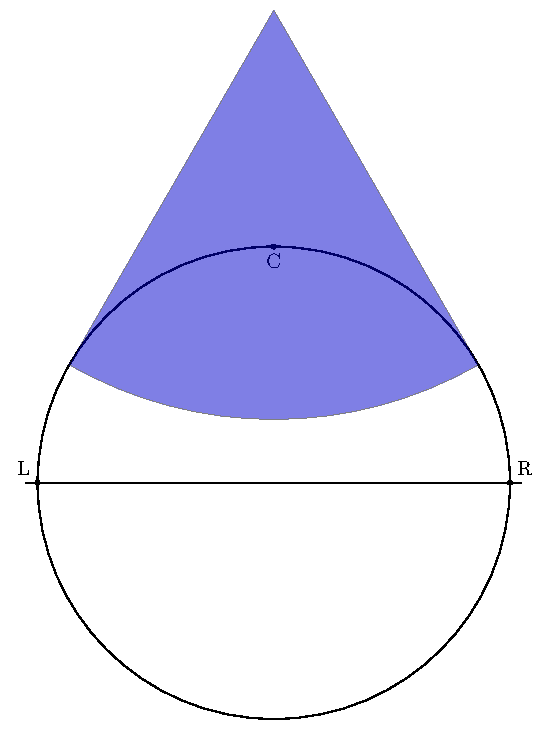
\includegraphics[height=8cm]{CAPITOLI/_TIKZ/PANNING/pan-frontal}
        \caption[]{Sorgente con incidenza frontale.}
        \label{pan:frontal}
    \end{subfigure}%
    ~
    \begin{subfigure}[t]{0.45\textwidth}
        \centering
        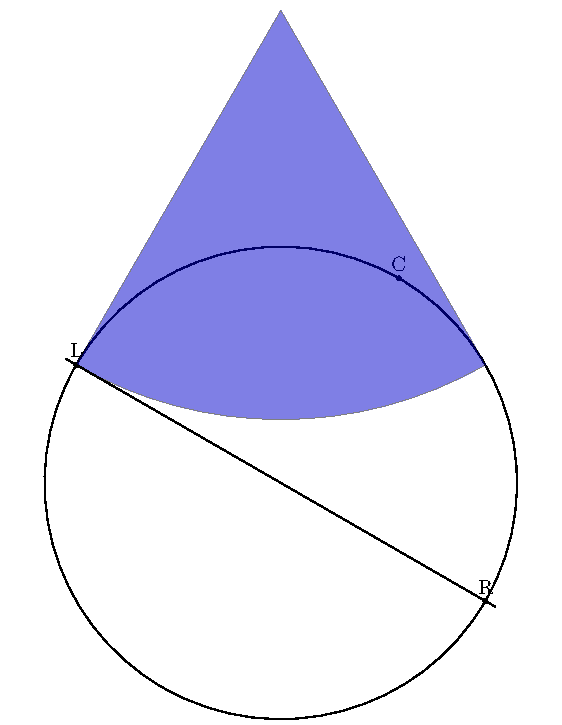
\includegraphics[height=8cm]{CAPITOLI/_TIKZ/PANNING/pan-left}
        \caption[]{Sorgente con incidenza laterale sinistra di 30 gradi.}
        \label{pan:left}
    \end{subfigure}
    \\
    \begin{subfigure}[t]{0.9\textwidth}
        \centering
        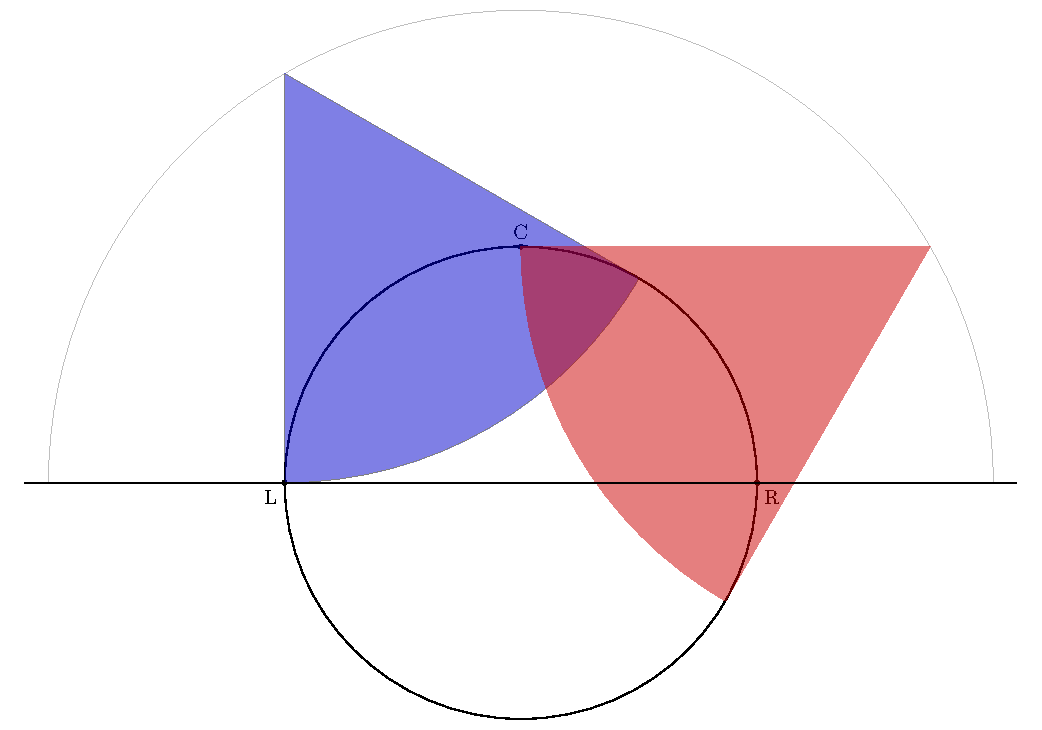
\includegraphics[height=8cm]{CAPITOLI/_TIKZ/PANNING/pan-both}
        \caption[]{Due sorgenti, una con incidenza laterale sinistra di 30 gradi,
        l'altra con incidenza laterale destra di 60 gradi.}
        \label{pan:both}
    \end{subfigure}
    \caption[]{La rotazione del \emph{PanPot} esegue una modifica della condizione
    di ascolto dell'ascoltatore, non un movimento della sorgente. Posizionando
    le singole sorgenti ci si pone in ascolto laterale, ruotati. Nella
    sovrapposizione di molteplici sorgenti il panorama risulta composto da
    ognuna di queste, con posizioni assolute ed angoli di incidenza relativi
    della testa.}
    \label{pan:all}
\end{figure*}

Un avvocato pronuncia la sua arringa in tribunale parlando ad alta voce,
camminando, rimbalzando tra destra e sinistra. La voce si propaga nello spazio
ed è inevitabile che se ne percepisca la variazione topologica, morfologica in
relazione con le caratteristiche architettoniche: a sinistra della stanza c'è
una parete di finestre, a destra un muro in cemento. Pur non avendo velocità
sufficiente ad innescare l'effetto doppler, la sua continua variazione di
posizione corrisponde ad una continua variazione di rapporto con l'ambiente che
lo circonda, in relazione ad ogni infinto punto di ascolto all'interno della
stanza. In altre parole, quel movimento assume significati diversi relativi al
punto di ascolto. Dovendo simulare lo stesso effetto mediante l'azione sul panpot, otterremmo la
variazione di posizione della voce nello spazio, ma non la sua relazione con lo
spazio.



Il \emph{panpot}, nella sua capacità di descrizione della relazione tra i canali
che ricevono i suoi segnali, non muove la sorgente nello spazio, ma regola la
posizione della sorgente stessa in relazione al nostro punto di ascolto. In
altri termini il \emph{panner} non regola il movimento della sorgente, ma la
rotazione della testa in relazione ad essa. Il \emph{panner}, muove langolo di
incidenza del suono, ruota la testa, nei confronti della sorgente immobile.

Ogni \emph{panner} ha un'architettura interna che determina la quantità e la
condizione del segnale sorgente per ogni canale di destinazione. I più semplici
suddividono i segnali audio nei due canali sinistro e destro, attraverso un
opportuno controllo di guadagno (volume) discreto. La distribuzione dell'energia
tra i due canali è chiamata legge ed è descrivibile con una funzione matematica.

Come descritto da Blumlein, la sola variazione di ampiezza nella
rappresentazione del panorama stereofonico rappresenta una parte nella complessa
soddisfazione della percezione binaurale, non disegna l'intero meccanismo.
Per questo motivo, prima di descrivere i sistemi di panning di ampiezza, che
sono universalmente implementati su tutti i mixer del pianeta, è più opportuno
riprendere da dove egli stesso è partito. La visione di Blumlein fu ripresa in
seguito da Michael Gerzon, negli anni settanta, per sviluppare la tecnologia
\emph{ambisonic}, la quale rimane un atto di descrizione del mondo sonoro
percepito e riprodotto, nell'evoluzione del concetto di stereofonia, completamente diverso
da quello che commercialmente si è diffuso ed imposto, per il semplice tentativo
di colmare il divario con il regno acustico.

\begin{quote}
The ears and brain localize sounds according to many different mechanisms. Among
the most important cues used are low-frequency interaural phase (applicable up
to around $2KHz$, but dominant below $700Hz$) and localization by
amplitude differences between the two ears, predominantly above about
$1KHz$. While other cues are also important, we have found that satisfying
both these cues, and making them mutually consistent for central listener facing
in any direction, leads to particularly robust and reliable localization
quality.\footnote{\cite{mg92pdmsss} - Le orecchie e il cervello localizzano i
suoni secondo molti meccanismi diversi. Tra i segnali più importanti utilizzati
vi sono la fase interaurale a bassa frequenza (applicabile fino a circa $2KHz$,
ma dominante al di sotto di $700Hz$) e la localizzazione mediante
differenze di ampiezza tra le due orecchie, prevalentemente al di sopra di
circa $1KHz$. Sebbene anche altri segnali siano importanti, abbiamo
scoperto che soddisfare entrambi questi segnali e renderli reciprocamente
coerenti per l'ascoltatore centrale rivolto verso qualsiasi direzione, porta
a una qualità di localizzazione particolarmente solida e affidabile.}
\end{quote}

%%%%%%%%%%%%%%%%%%%%%%%%%%%%%%%%%%%%%%%%%%%%%%%%%%%%%%%%%%%%%%%%%%%% SUBSECTION
%%%%%%%%%%%%%%%%%%%%%%%%%%%%%%%%%%%%%%%%%%%%%%%%%%%%%%%%%%%%%%%%%%%%%%%%%%%%%%%%
\subsection{Sul concetto di \emph{Figura Polare}}
\label{sec:polarplot}

La figura polare di un microfono è la rappresentazione grafica su di un piano,
nel sistema di coordinate polari, della sensibilità in funzione dell'angolo di
incidenza del suono sulla membrana. Questo tipo di figura polare si presenta
come una linea curva chiusa (o insieme di più linee di questo tipo, tipicamente
associate alle ampiezze polari in risposta a diverse frequenze). In presenza di
un’unica curva la si intende riferita ad una frequenza di $1KHz$ in rappresentazione
di un valore generico di intensità di risposta del microfono stesso,
e come tale fornisce una rapida indicazione visiva di come l'intensità di
risposta sia geometricamente distribuita intorno
al microfono stesso.

\begin{figure}[h]
\centering
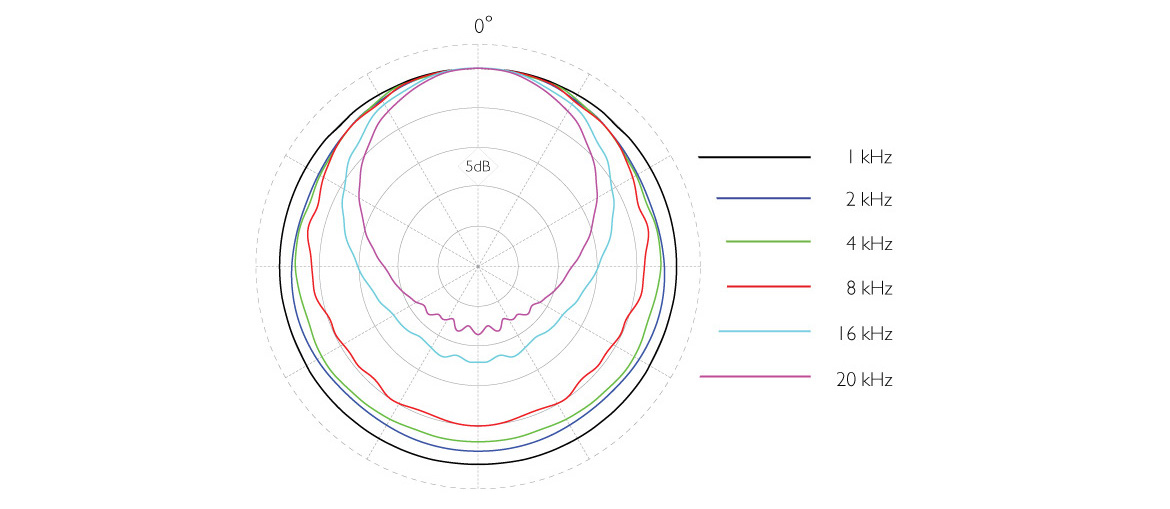
\includegraphics[width=0.99\columnwidth]{CAPITOLI/1000/IMG/4006A-ddicate-4006A-Omni-Microphone-polar-pattern.jpg}
\caption[]{Risposta polare in frequenza del microfono \emph{DPA 4006A}.}% \url{https://www.dpamicrophones.com/pencil/4006-omnidirectional-microphone}.}
\label{pol:dpa4006}
\end{figure}

\begin{figure}[t]
\centering
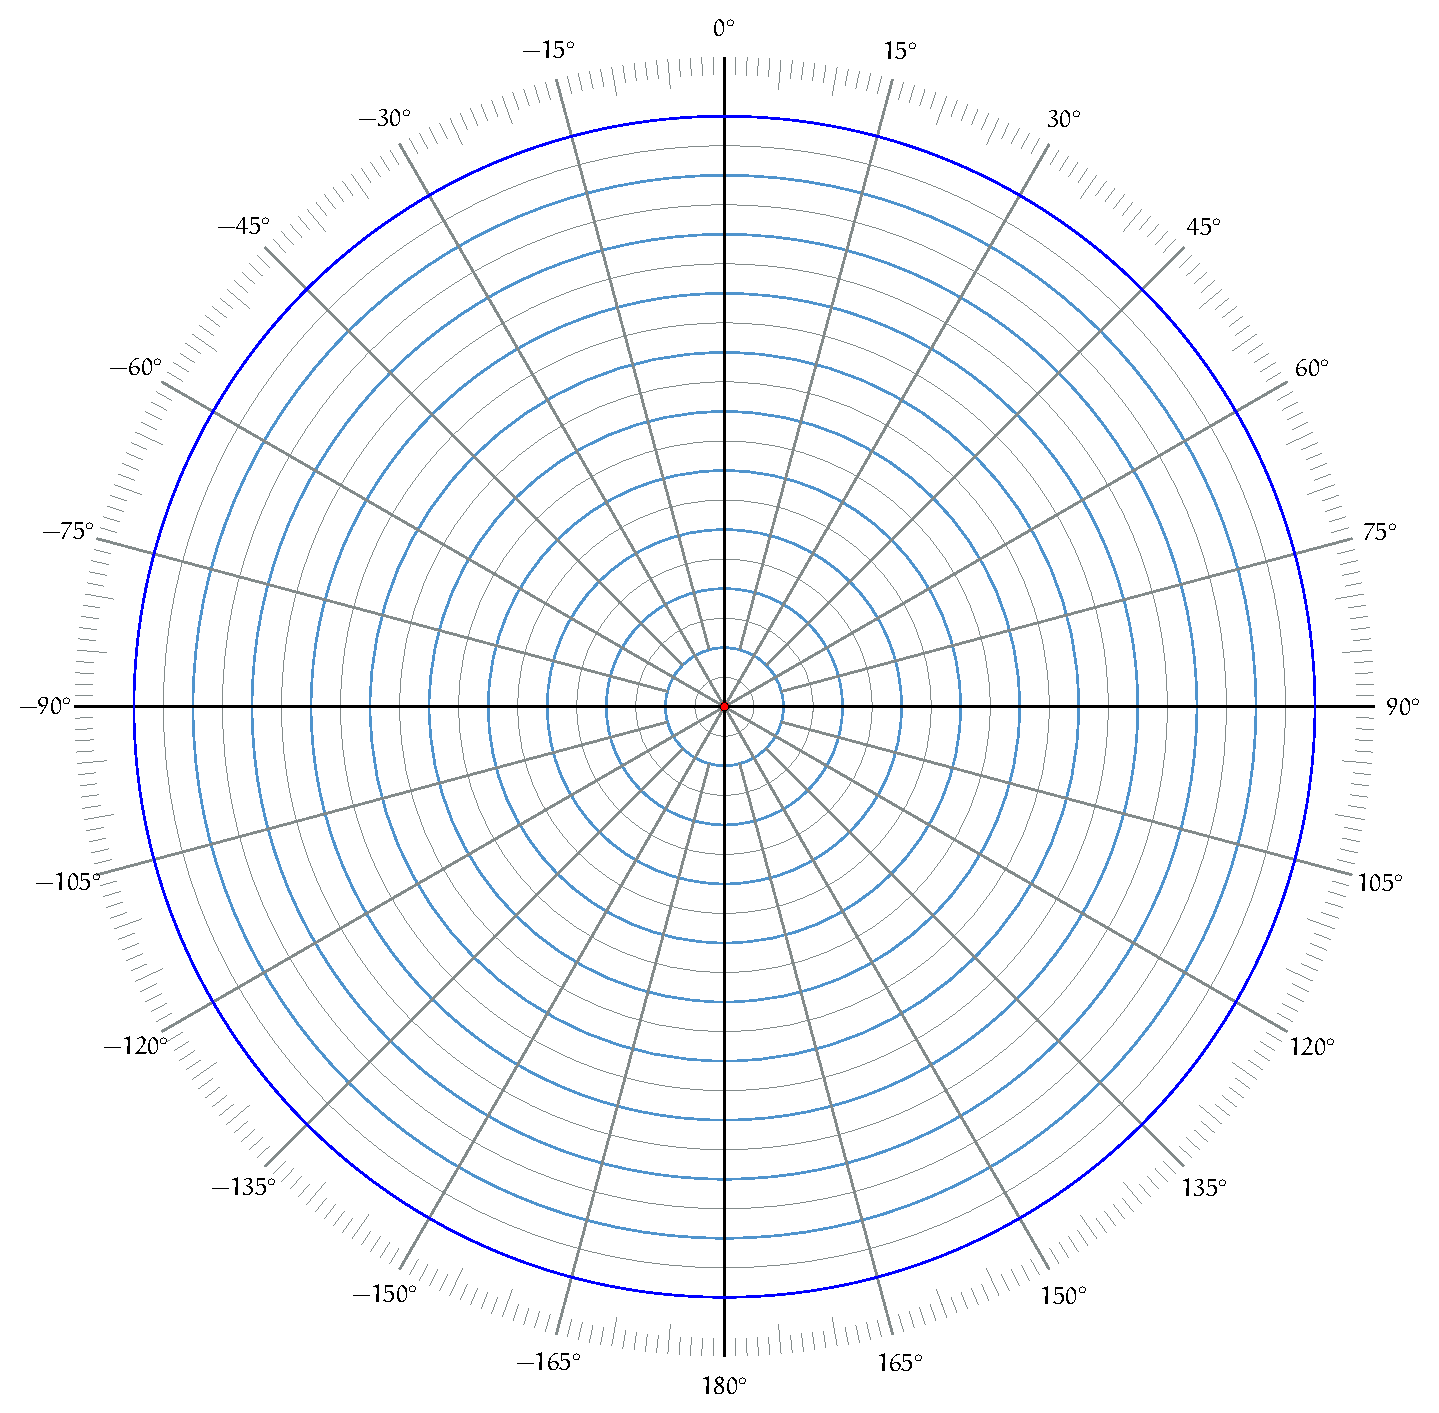
\includegraphics[width=0.99\columnwidth]{microphone-polar-patterns/omni}
\caption[]{Rappresentazione ideale del microfono a pressione mediante la sua
equazione polare: $ndp = 1(x)$ (non-directional pressure). La figura polare
descrive una risposta in fase lineare per ogni angolo di inncidenza.}
\label{polar:omni}
\end{figure}

In un sistema polare ciascun punto è
determinato da una distanza, da un punto di riferimento, ed un angolo, da una
direzione di riferimento. Nel caso di una figura polare di un microfono, il
punto di riferimento è l'origine, il centro del piano e la direzione di
riferimento è il fronte, ovvero l'asse di puntamento frontale del microfono. Per
questa ragione la figura polare del microfonico presenta l'angolo zero
nel nord del piano, si muove angolarmente verso sinistra per angoli
negativi e verso destra per angoli positivi. Il movimento angolare, denominato
\emph{azimuth} è espresso in radianti $(-\pi,\pi)$ ed una eventuale indicazione in
gradi può essere connvertita in radianti mediante l'equazione $deg = \pi/180$,
con valori negativi a sinistra e positivi a destra.

Un segnale nella sua oscillazione espressa nella variazione di ampiezza
attorno allo zero potrebbe essere derivato da qualsiasi tipo di microfono senza
un significato particolare. Potrebbe essere generato elettricamente da un
microfono con modello polare particolare o generato sinteticamente secondo equazioni polari, senza
alcuna rilevanza specifica in termini di descrizione dell'andamento di ampiezza.
La provenienza polare, la forma che assume la fase del segnale, diventa rilevante nel confronto tra segnali.

La figura polare ideale di un microfono che non trasferisce informazioni relative
alle variazioni dell'angolo di incidenza del suono è definita dall'equazione:

\begin{equation}
ndp = 1(x)
\label{eq:omni}
\end{equation}

Un microfono di questo tipo descrive esclusivamente variazioni di ampiezza
derivate della variazione di pressione dell'aria, motivo per cui è definito
microfono a pressione, e risponde alla figura polare \emph{non-direzionale}, anche se
nel mercato dei microfoni si è imposto con il nome \emph{omni-direzionale}.

La membrana di un microfono di questo tipo è stesa, come la pelle di un tamburo a fusto chiuso.
Il dispositivo oscilla in presenza di variazioni di pressione provenienti esclusivamente dall’esterno,
essendo la parte interna a pressione costante. Idealmente le variazioni di pressione sono indipendenti
dall’angolo di incidenza sulla membrana. Nella realtà fisica fisica la membrana
è sottoposta a fenomeni di diffrazione acustica che ne modificano la risposta polare in frequenza.
Le frequenze acute tendono a descrivere variazioni di sensibilità al variare
dell’angolo di incidenza del suono in relazione al fronte microfonico.
I fenomeni di diffrazione acustica avvengono in relazione alla presenza fisica
del microfono stesso nel campo sonoro che interferisce con la propagazione delle
onde sonore ad alta frequenza, ostacolandole.

La figura \ref{pol:dpa4006} rappresenta la curva polare di un ottimo microfono
omni-direzionale. Si può osservare che la caratteristica non-direzionalità di
percezione del suono è reale solo per un range di frequenze, mentre il microfono
inizia ad ad avere un carattere direzionale da circa per le frequenze acute.
Le frequenze gravi sotto a $1KHz$ non sono descritte singolarmente perché
assimilabili alla frequenza di riferimento di $1KHz$. Lo stesso microfono può essere
equipaggiato da correttori acustici per la ripresa sonora in campo libero. Lo
scopo di questi correttori acustici è proprio quello di avvicinare la resa del
microfono alla figura polare ideale non-direzionale, come mostrato in figura \ref{pol:dpa4006nose}.

\begin{figure}[h]
\centering
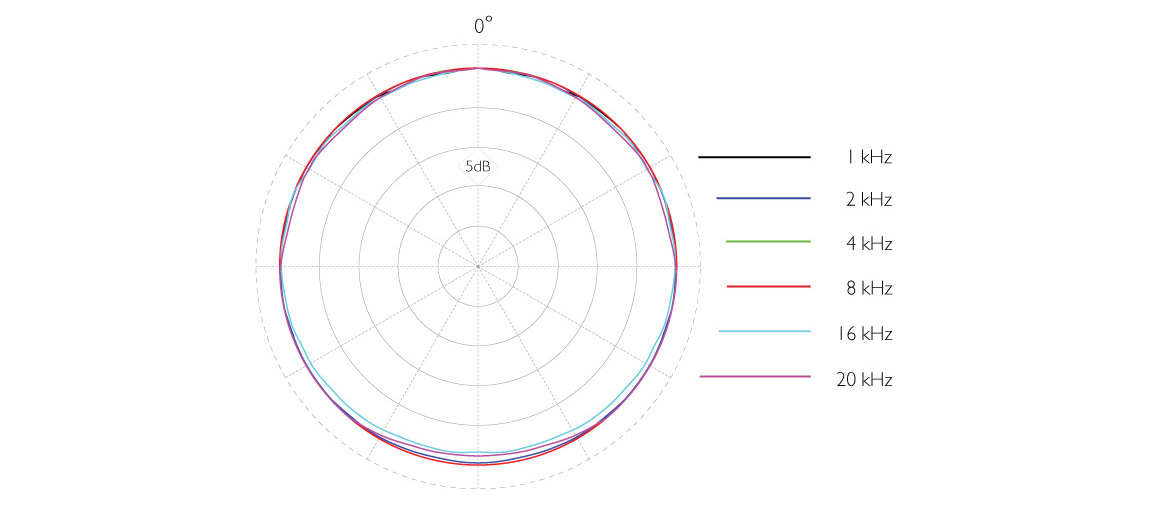
\includegraphics[width=0.99\columnwidth]{CAPITOLI/1000/IMG/4006A-ddicate-4006A-Omni-Microphone-polar-pattern-nose-cone-veritical.jpg}
\caption[]{Risposta polare in frequenza del microfono \emph{DPA 4006A} con \emph{Nose Cone AU0777}, microfono con posizionamento verticale.}% \url{https://www.dpamicrophones.com/pencil/4006-omnidirectional-microphone}.}
\label{pol:dpa4006nose}
\end{figure}

\begin{figure}[t]
\centering
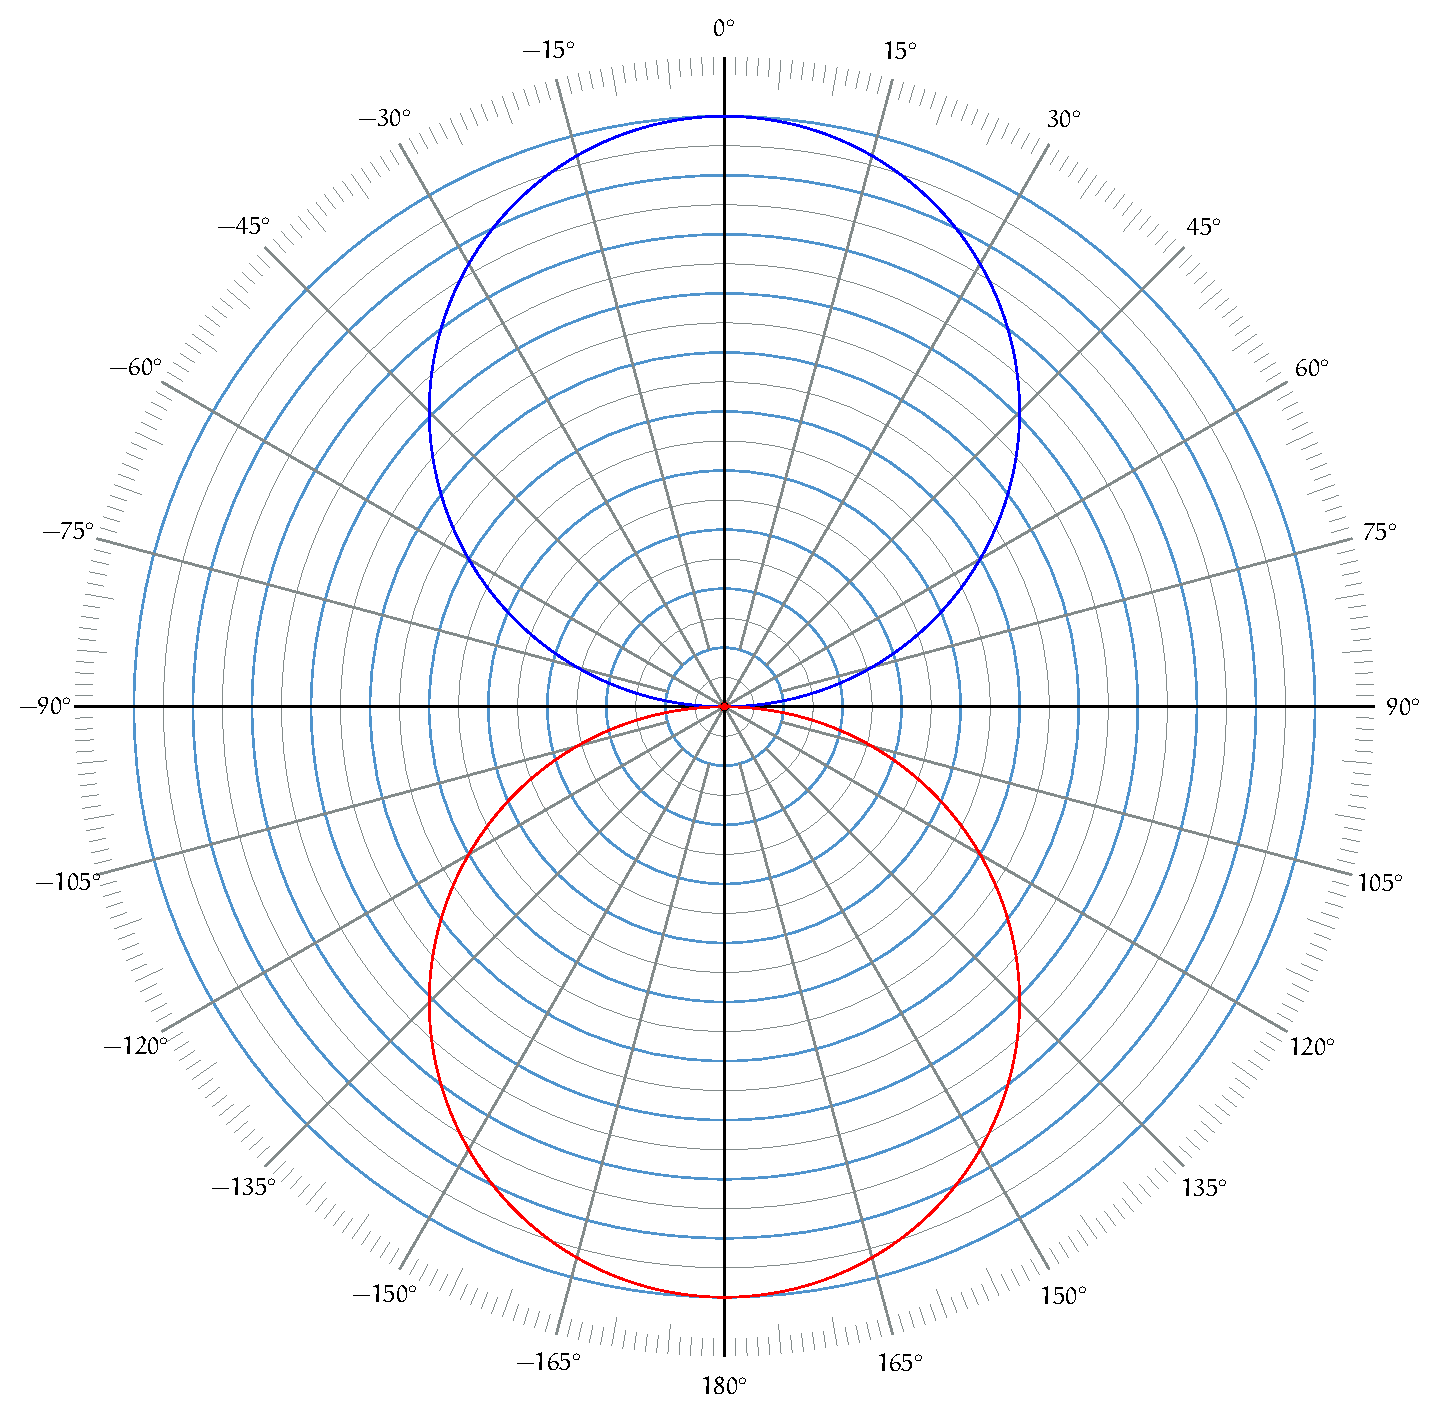
\includegraphics[width=0.99\columnwidth]{microphone-polar-patterns/fig8}
\caption[]{Rappresentazione ideale del microfono bidirezionale a gradiente di
pressione mediante la sua equazione polare: $bpg = x\cos\theta$
(\emph{bidirectional pressure gradient}). La figura polare descrive una risposta
in fase bipolare, positiva per angoli di incidenza frontali ($(-\pi/2,\pi/2)$),
negativa per angoli di incidenza posteriori ($[(-\pi,-\pi/2),(\pi/2,\pi)]$)}
\label{polar:fig8}
\end{figure}

\begin{figure}[t]
\centering
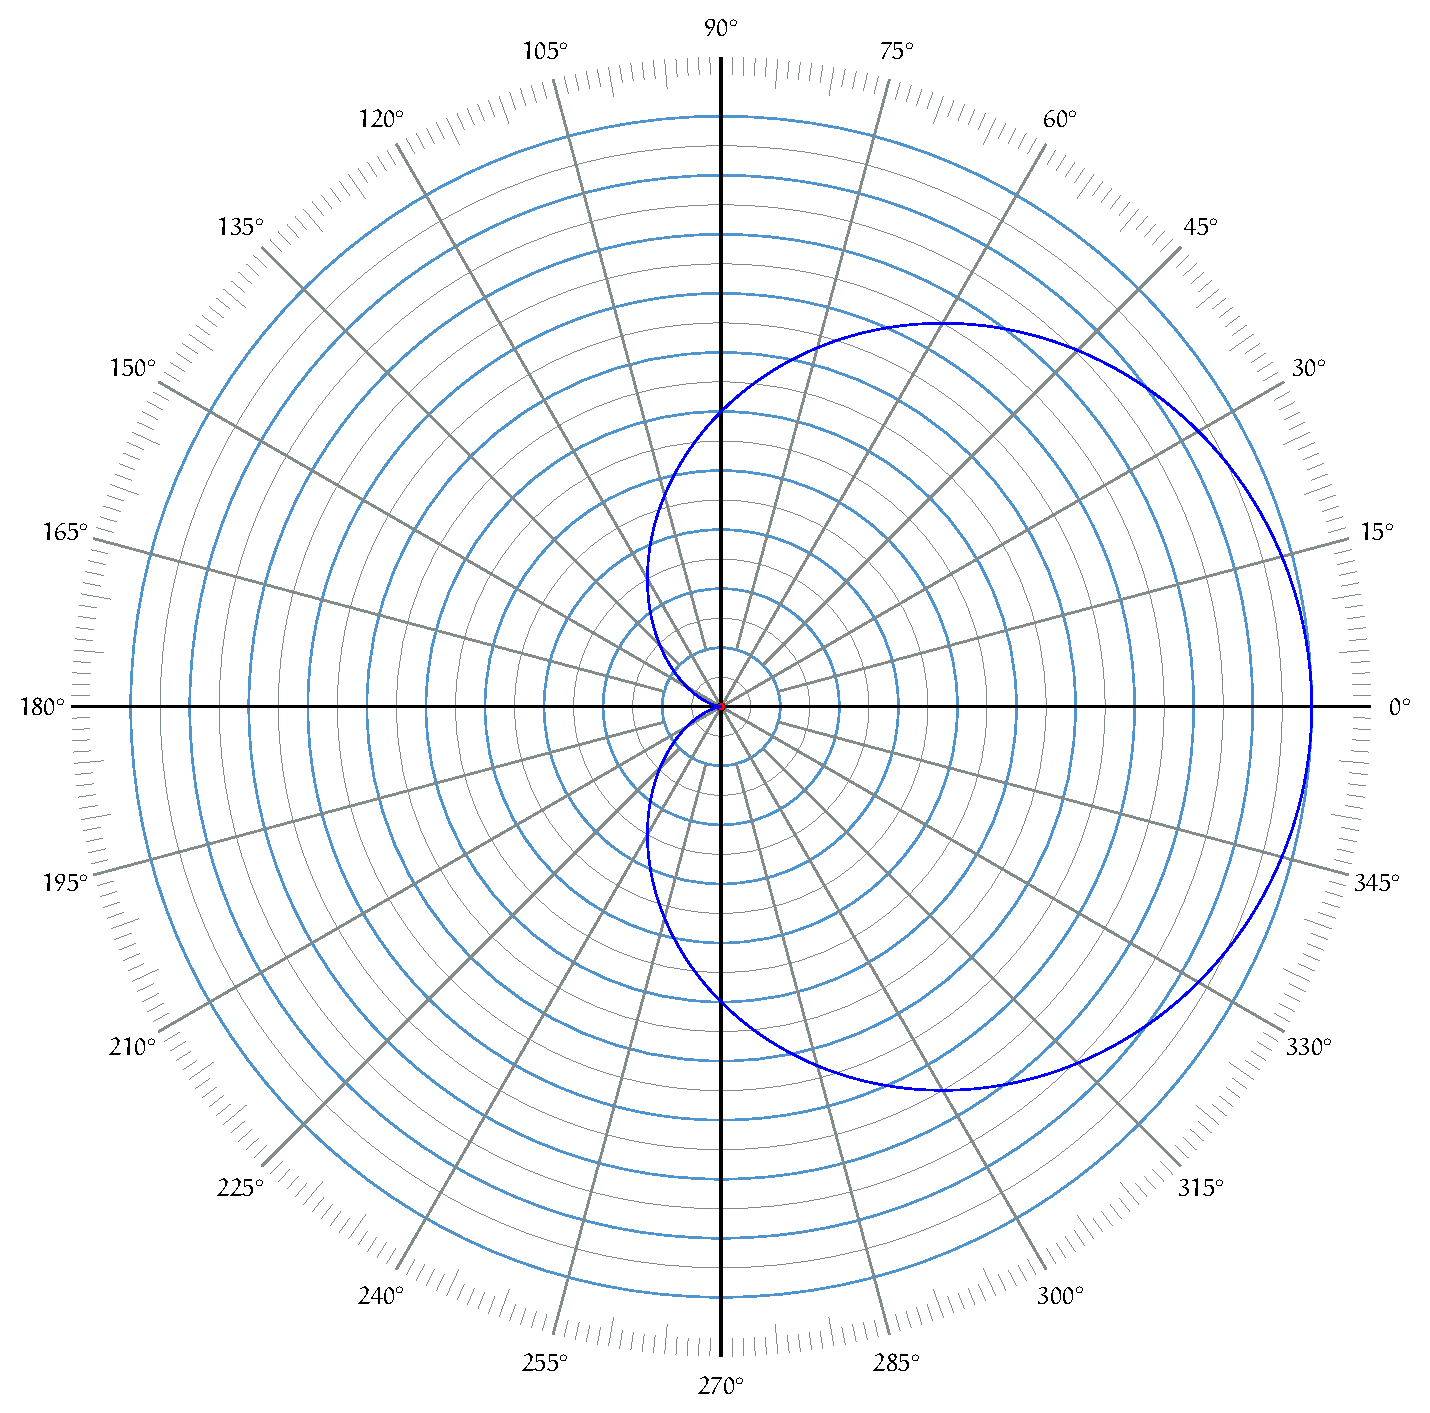
\includegraphics[width=0.99\columnwidth]{microphone-polar-patterns/cardioid}
\caption[]{Rappresentazione ideale del microfono direzionale cardioide a gradiente
di pressione mediante la sua equazione polare: $cpg = 0.5(x) + 0.5(x\cos\theta)$
(\emph{cardioid pressure gradient}). La figura polare descrive una risposta in
fase positiva non lineare per diversi angoli di inncidenza.}
\label{polar:cardioid}
\end{figure}

I microfoni che per cratteristiche costruttive presentano principi di direzionalità
vengono definiti \emph{microfoni a gradiente di pressione} in quanto la variazione
di pressione dell'aria è percepita in maniera diversa per angoli d'incidenza diversi.
Tra questi, il microfono bidirezionale denominato microfono a \emph{figura-8},
presenta una figura polare simmetrica fronte-retro, con punti di attenuazione
massima a $\pm90°$. Tali microfoni hanno uguale sensibilità per i suoni
provenienti dal fronte e dal retro, mentre tendono ad annullare i suoni di
provenienza laterale. La doppia direzionalità caratterizza una doppia polarità
in quanto i segnali generati da angoli di incidenza posteriori sono caratterizzati da
una fase negativa.

\begin{equation}
bpg = x\cos\theta
\label{eq:fig8}
\end{equation}

La prima differenza rilevante tra un'equazione del modello polare non
direzionale (\ref{eq:omni}) e una direzionale (\ref{eq:fig8}) è la
presenza del coefficiente angolare. L'angolo \emph{theta} nell'equazione
(\ref{eq:fig8}) descrive la direzione polare di puntamento del microfono bidirezionale
espressa in radianti che, nel caso specifico, corrisponde a zero radianti. Il valore di
$x$ esprime la variazione d'ampiezza del segnale relativo alla variazione di pressione.

In termini ideali la somma tra figure polari produce figure risultanti aventi caratteri
di entrambe le figure originarie. In questo modo, sommando pari quantità di componenti
non-direzionale e bipolare, si ottiene una figura polare intermedia che prende il
nome di figura cardioide.

\begin{equation}
cpg = 0.5(x) + 0.5(x\cos\theta)
\label{eq:cardioid}
\end{equation}

Il microfono cardioide appartiene, come il microfono bidirezionale, alla tipologia
gradiente di pressione (\emph{cpg}), in quanto la produzione del segnale elettrico è condizionata
dall'angolo di incidenza.

La figura polare cardioide presenta la sola polarità positiva, una spiccata
sensibilità frontale ed una progressiva riduzione di sensibilità al variare dell'angolo
di incidennza.

Cardioidi e altre figure polari comuni del primo ordine, come anche ogni
sfumatura di forma tra di loro, sono prodotte con diversi coefficienti di peso
tra la pressione non-direzionale e gradiente di pressione bidirezionale,
come in tabella \ref{tab:polarcoef}. Ogni figura direzionale prodotta può avere
un proprio angolo di punatamento intorno a $2\pi$ radianti.

\vfill\null

\begin{figure}[hb]
\centering
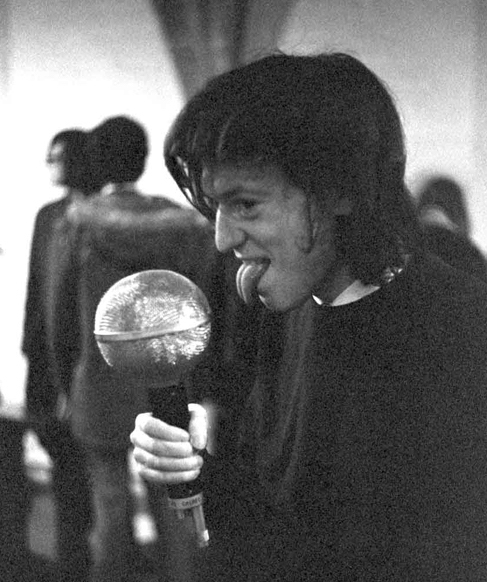
\includegraphics[width=0.99\columnwidth]{CAPITOLI/1000/IMG/MAG-licking-G-web.jpg}
\caption[]{Michael Gerzon}
\label{ph:mg1}
\end{figure}

\clearpage

\begin{table}[ht]
%\scriptsize
\caption[]{Coefficienti di pressione \emph{non-direzionale} e gradiente di pressione
\emph{bidirezionale} per la descrizione dei modelli polari intermedi, del primo ordine.
Dove $x$ è la variazione d'ampiezza del segnale relativa alla pressione in
ingresso e $\theta$ l'angolo di incidenza}
\begin{center}
\begin{tabular}{rrcll}
\textbf{Polar Pattern} & \textbf{NDP} & : & \textbf{BPG} &\\
\hline
non-direzionale & $1(x)$       &     &                      &
 \multirow{4}{*}{\begin{minipage}{.25\textwidth}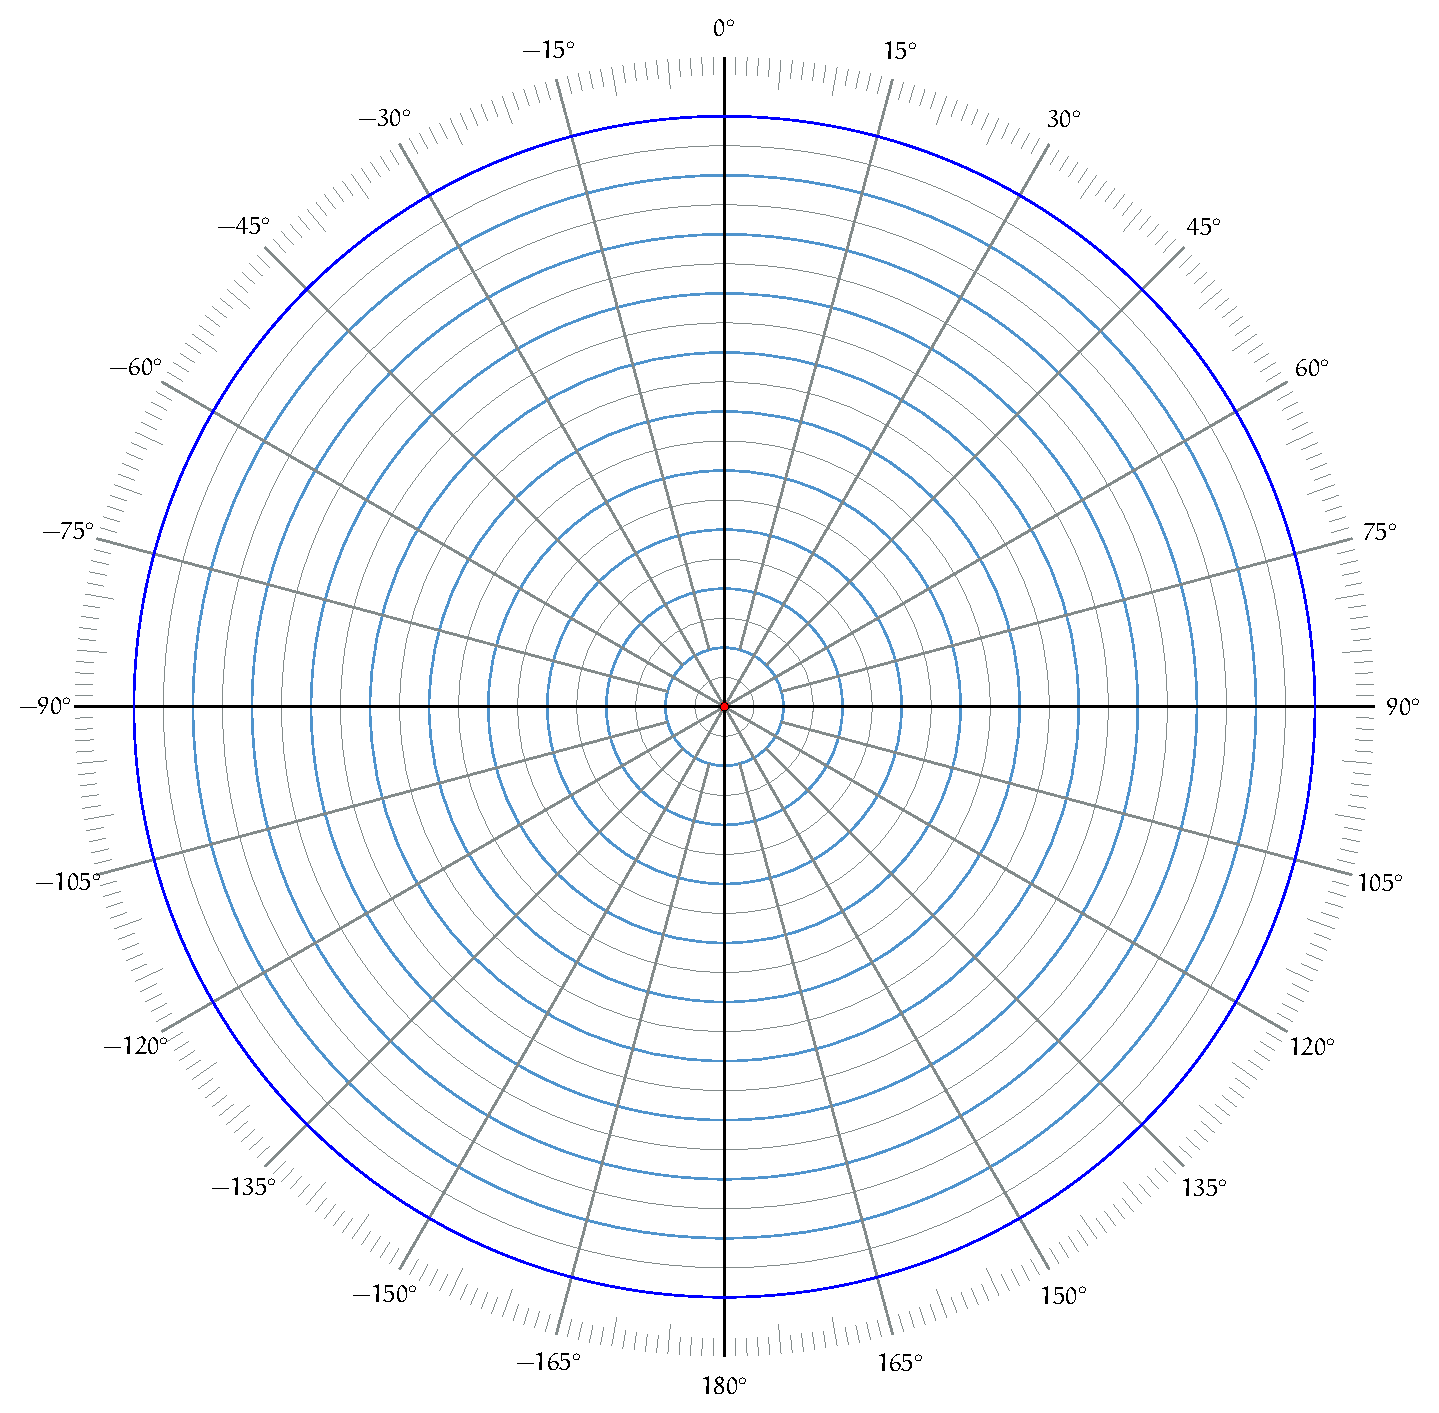
\includegraphics[width=\linewidth]{microphone-polar-patterns/omni}\end{minipage}} \\
                & $1$          & $+$ & $0$                  & \\
                & $0dB$        & $+$ & $-\infty$         & \\ %20*log10(g)
& \\
\hline
subcardioide    & $0.75(x)$    & $+$ & $0.25(x\cos\theta)$  &
 \multirow{4}{*}{\begin{minipage}{.25\textwidth}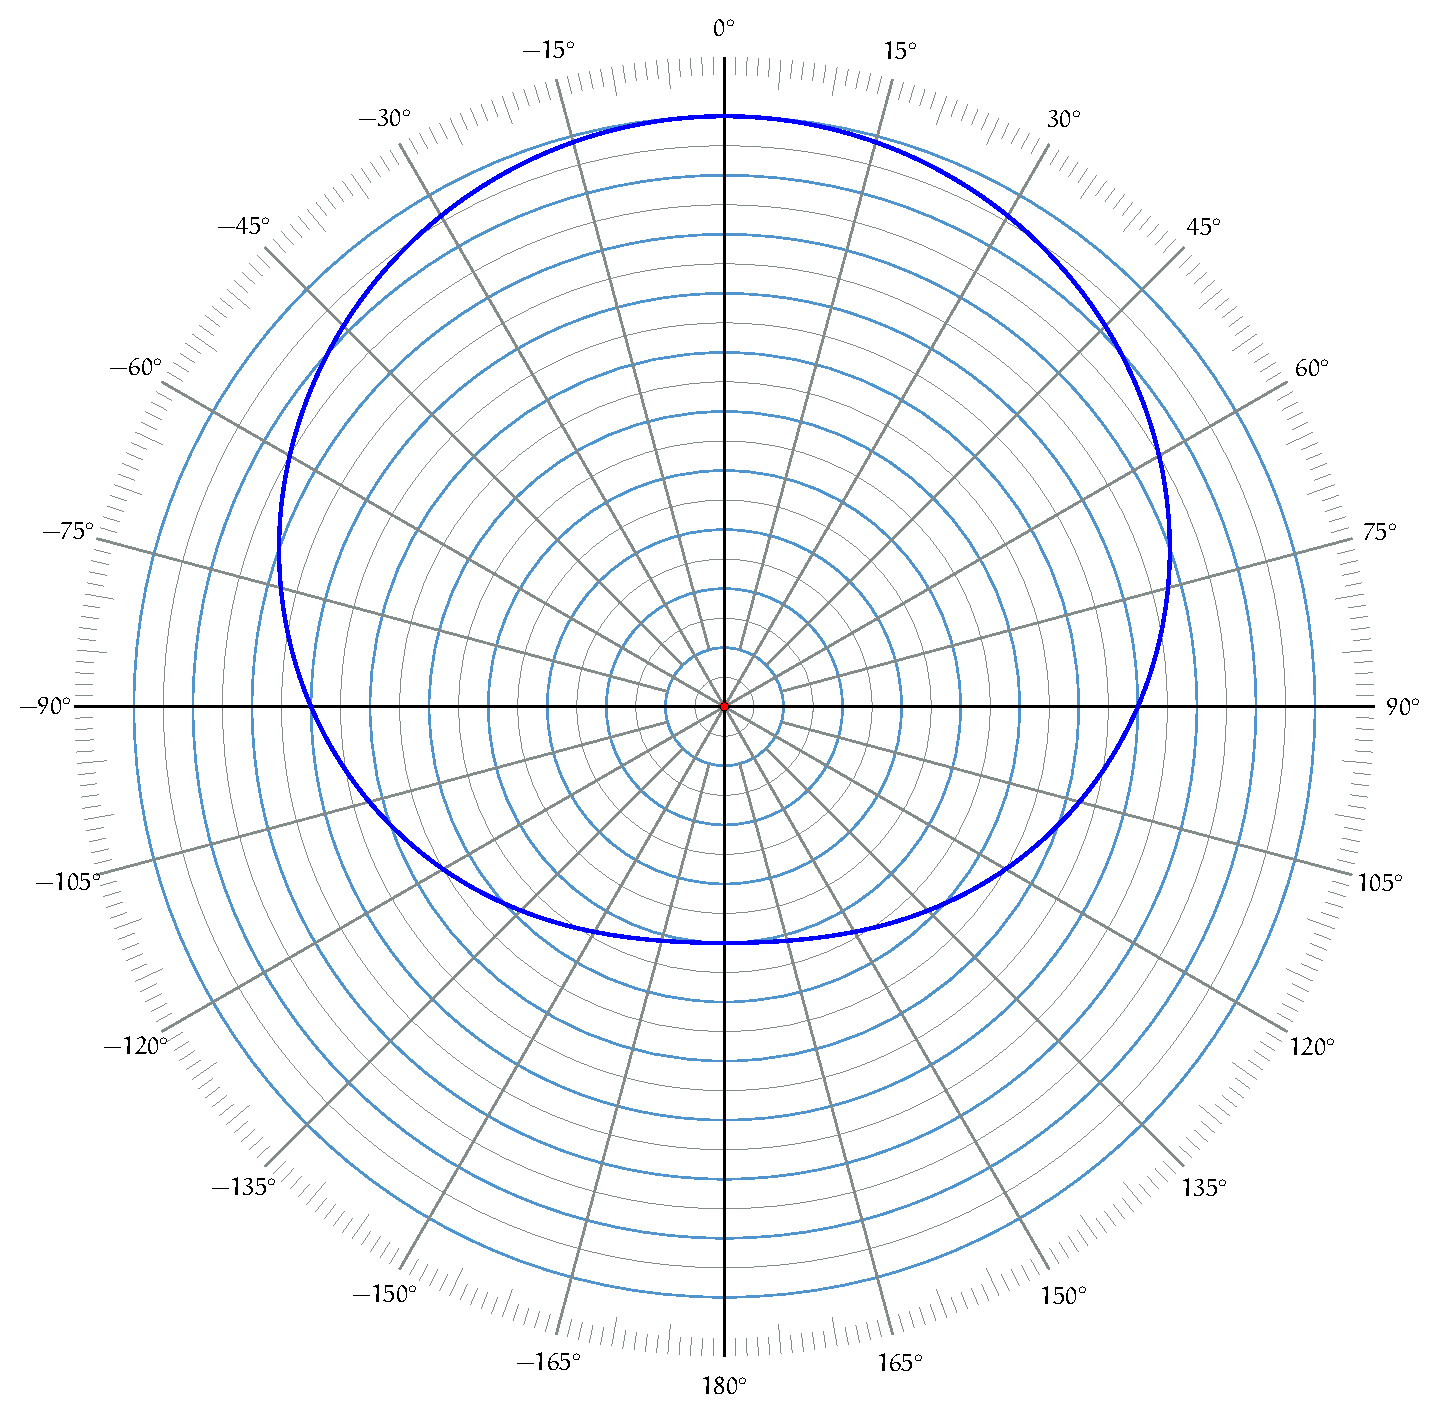
\includegraphics[width=\linewidth]{microphone-polar-patterns/subcardioid}\end{minipage}} \\
                & $0.75$       & $+$ & $0.25$               & \\
                & $-2.75dB$    & $+$ & $-12.05dB$           & \\
& \\
\hline
cardioide       & $0.5(x)$     & $+$ & $0.5(x\cos\theta)$   &
 \multirow{4}{*}{\begin{minipage}{.25\textwidth}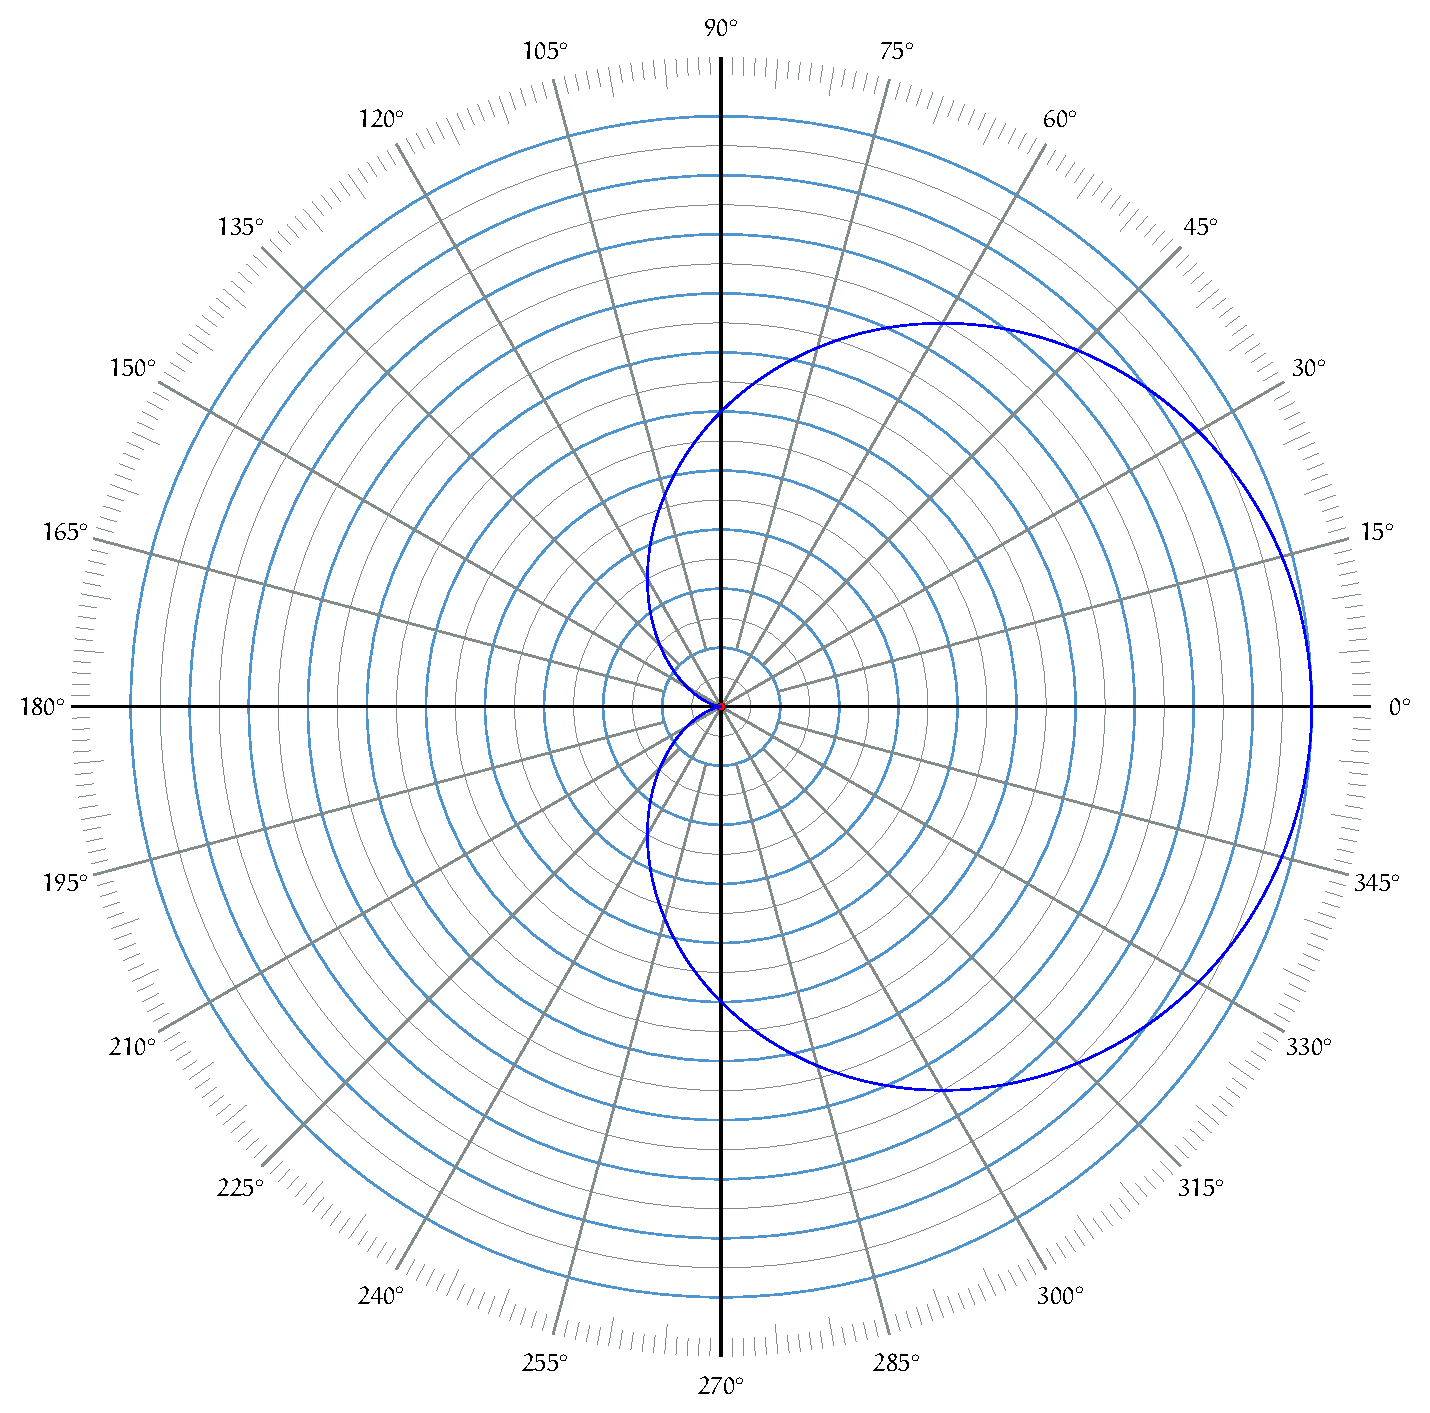
\includegraphics[width=\linewidth]{microphone-polar-patterns/cardioid}\end{minipage}} \\
                & $0.5$        & $+$ & $0.5$                & \\
                & $-6.02dB$    & $+$ & $-6.02dB$            & \\ %20*log10(g)
& \\
\hline
supercardioide  & $0.37(x)$    & $+$ & $0.63(x\cos\theta)$  &
 \multirow{4}{*}{\begin{minipage}{.25\textwidth}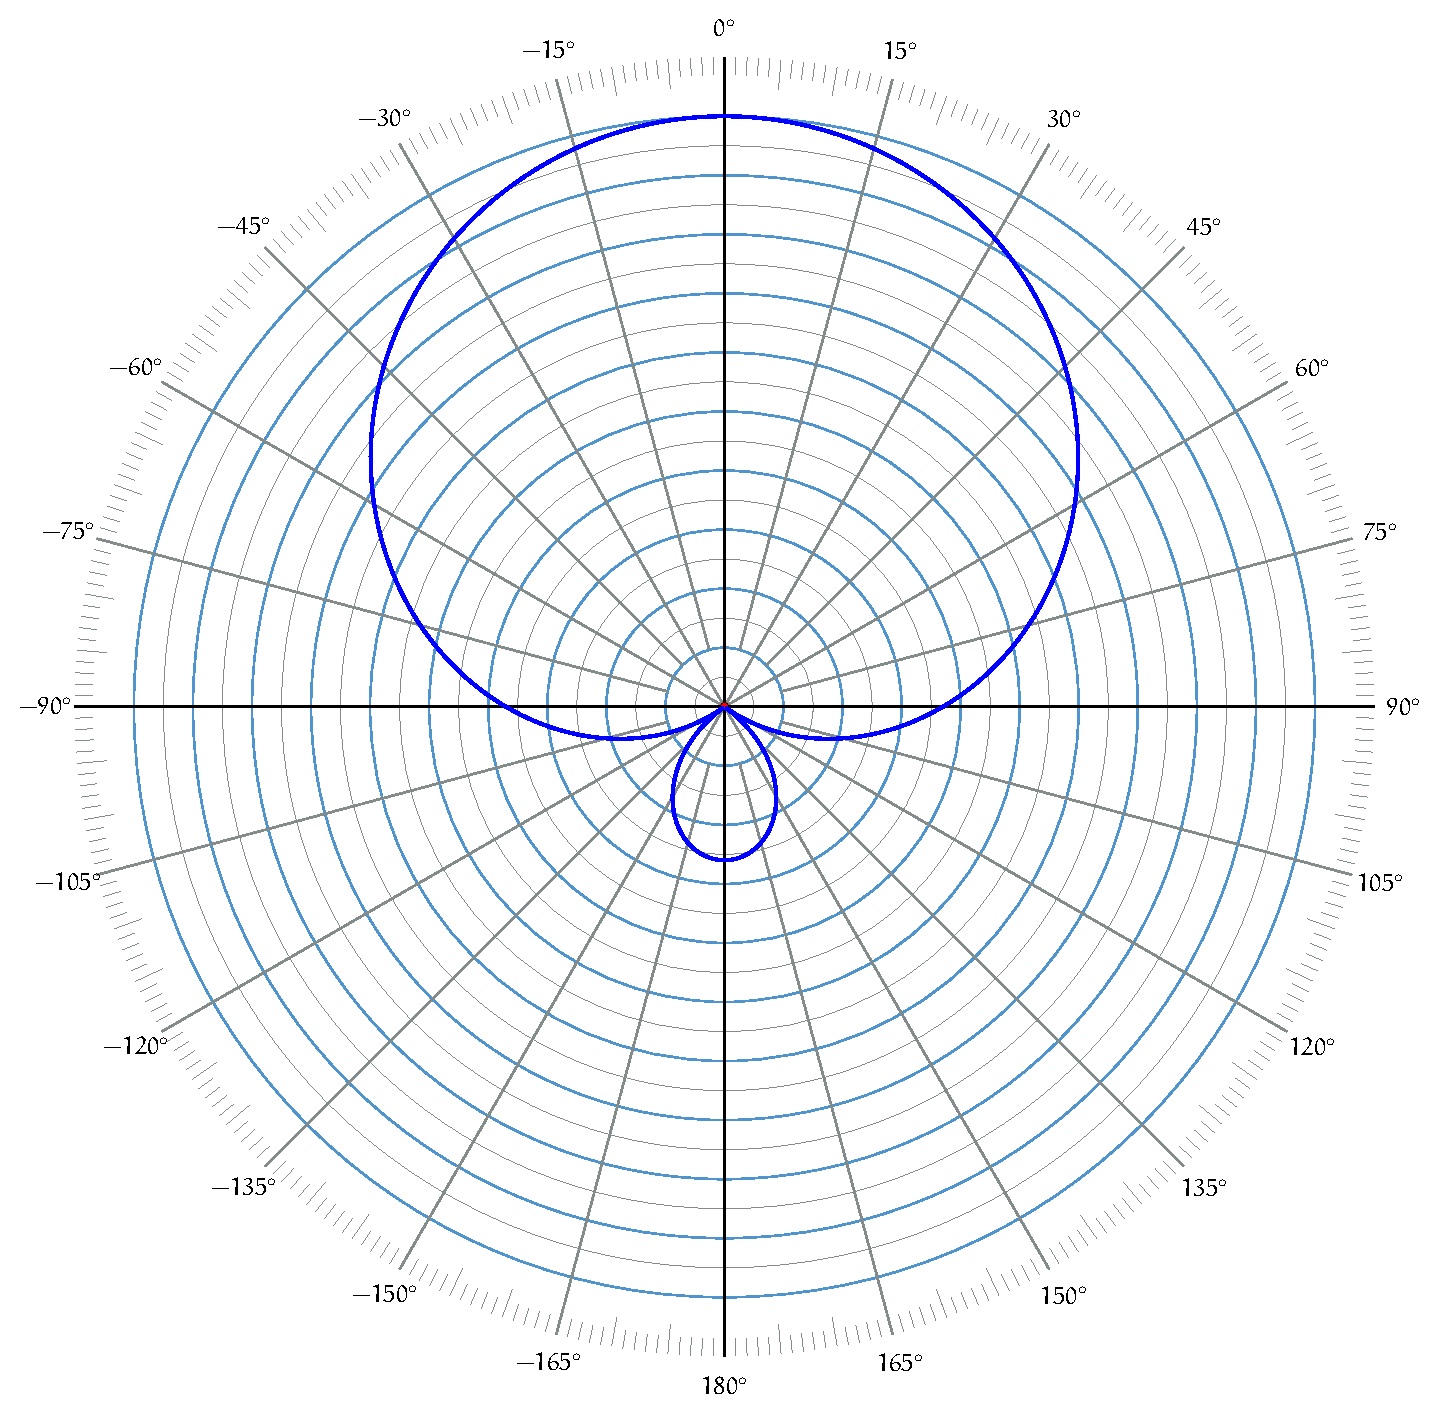
\includegraphics[width=\linewidth]{microphone-polar-patterns/supercardioid}\end{minipage}} \\
                & $0.37$       & $+$ & $0.63$               & \\
                & $-8.64dB$    & $+$ & $-4.01dB$            & \\ %20*log10(g)
& \\
\hline
ipercardioide   & $0.25(x)$    & $+$ & $0.75(x\cos\theta)$  &
 \multirow{4}{*}{\begin{minipage}{.25\textwidth}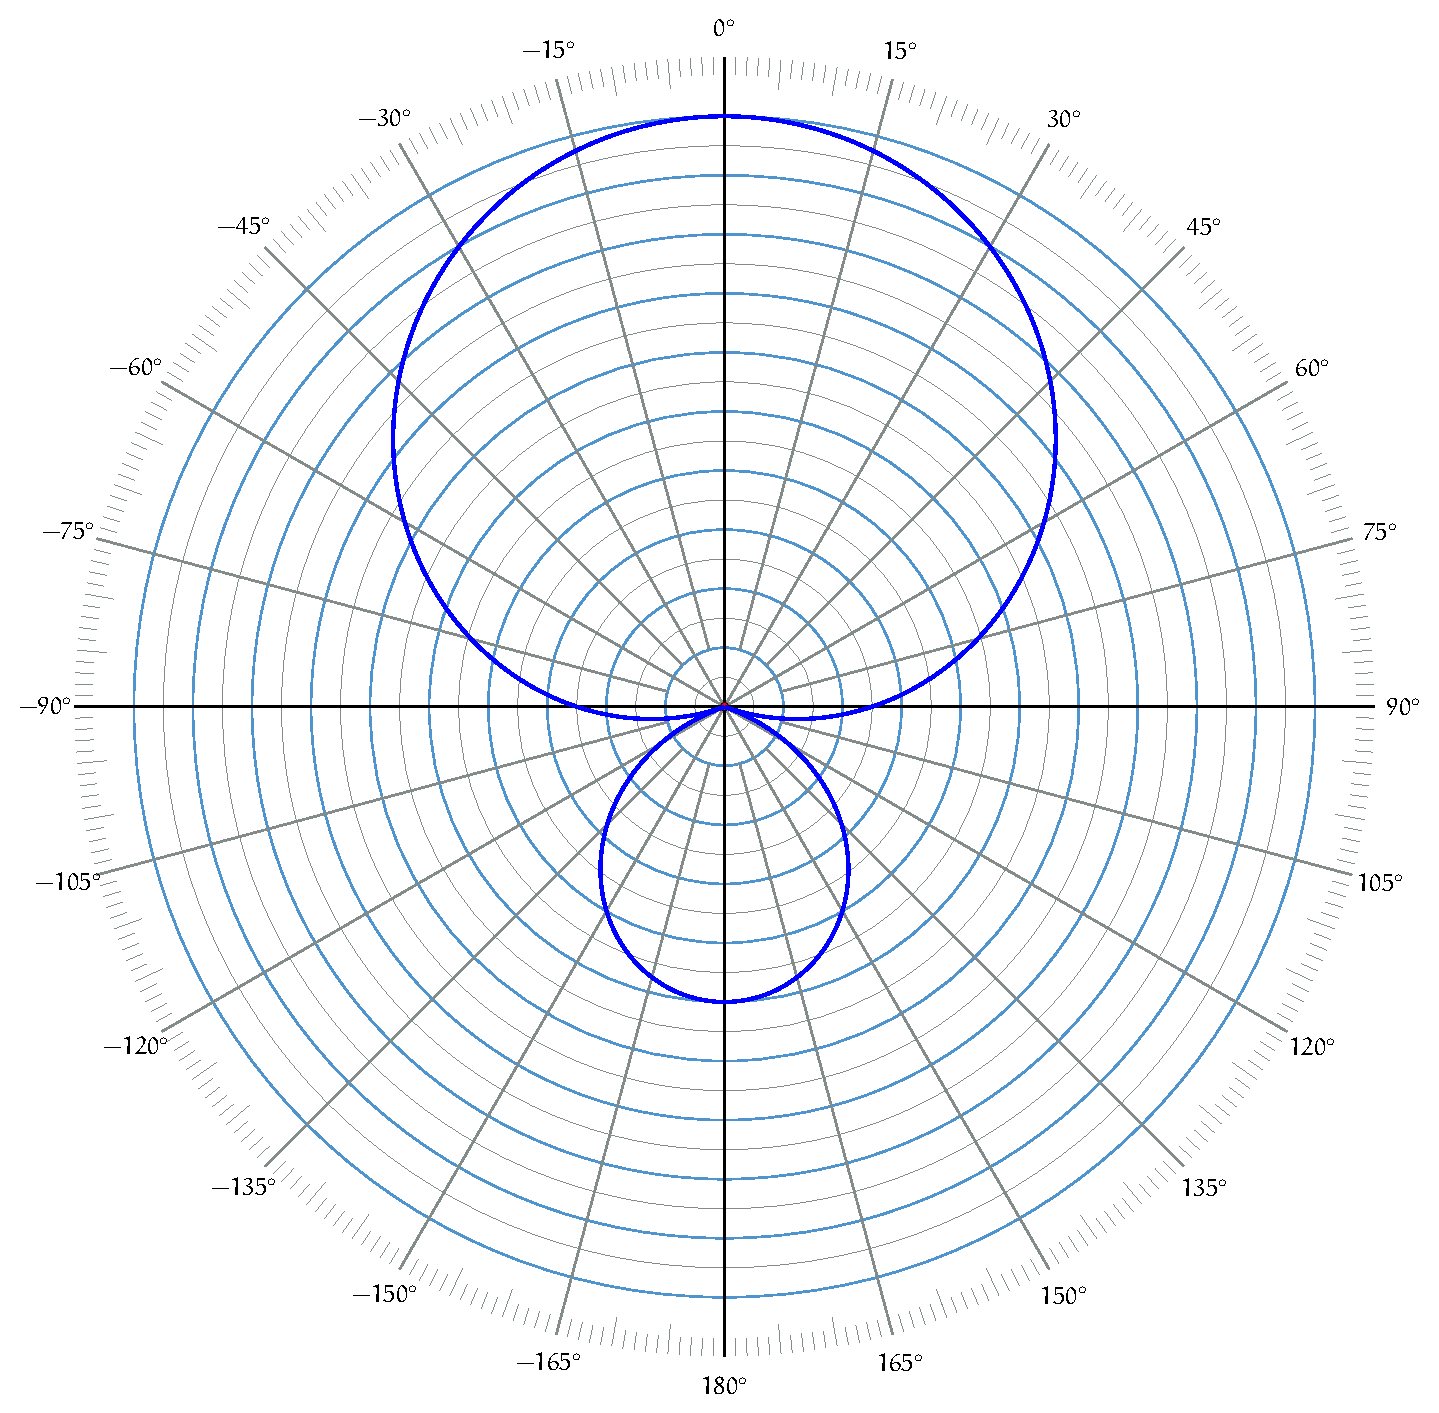
\includegraphics[width=\linewidth]{microphone-polar-patterns/hypercardioid}\end{minipage}} \\
                & $0.25$       & $+$ & $0.75$               & \\
                & $-12.05dB$ & $+$ & $-2.75dB$              & \\ %20*log10(g)
& \\
\hline
bidirezionale   &              &     & $1(x\cos\theta)$     &
 \multirow{4}{*}{\begin{minipage}{.25\textwidth}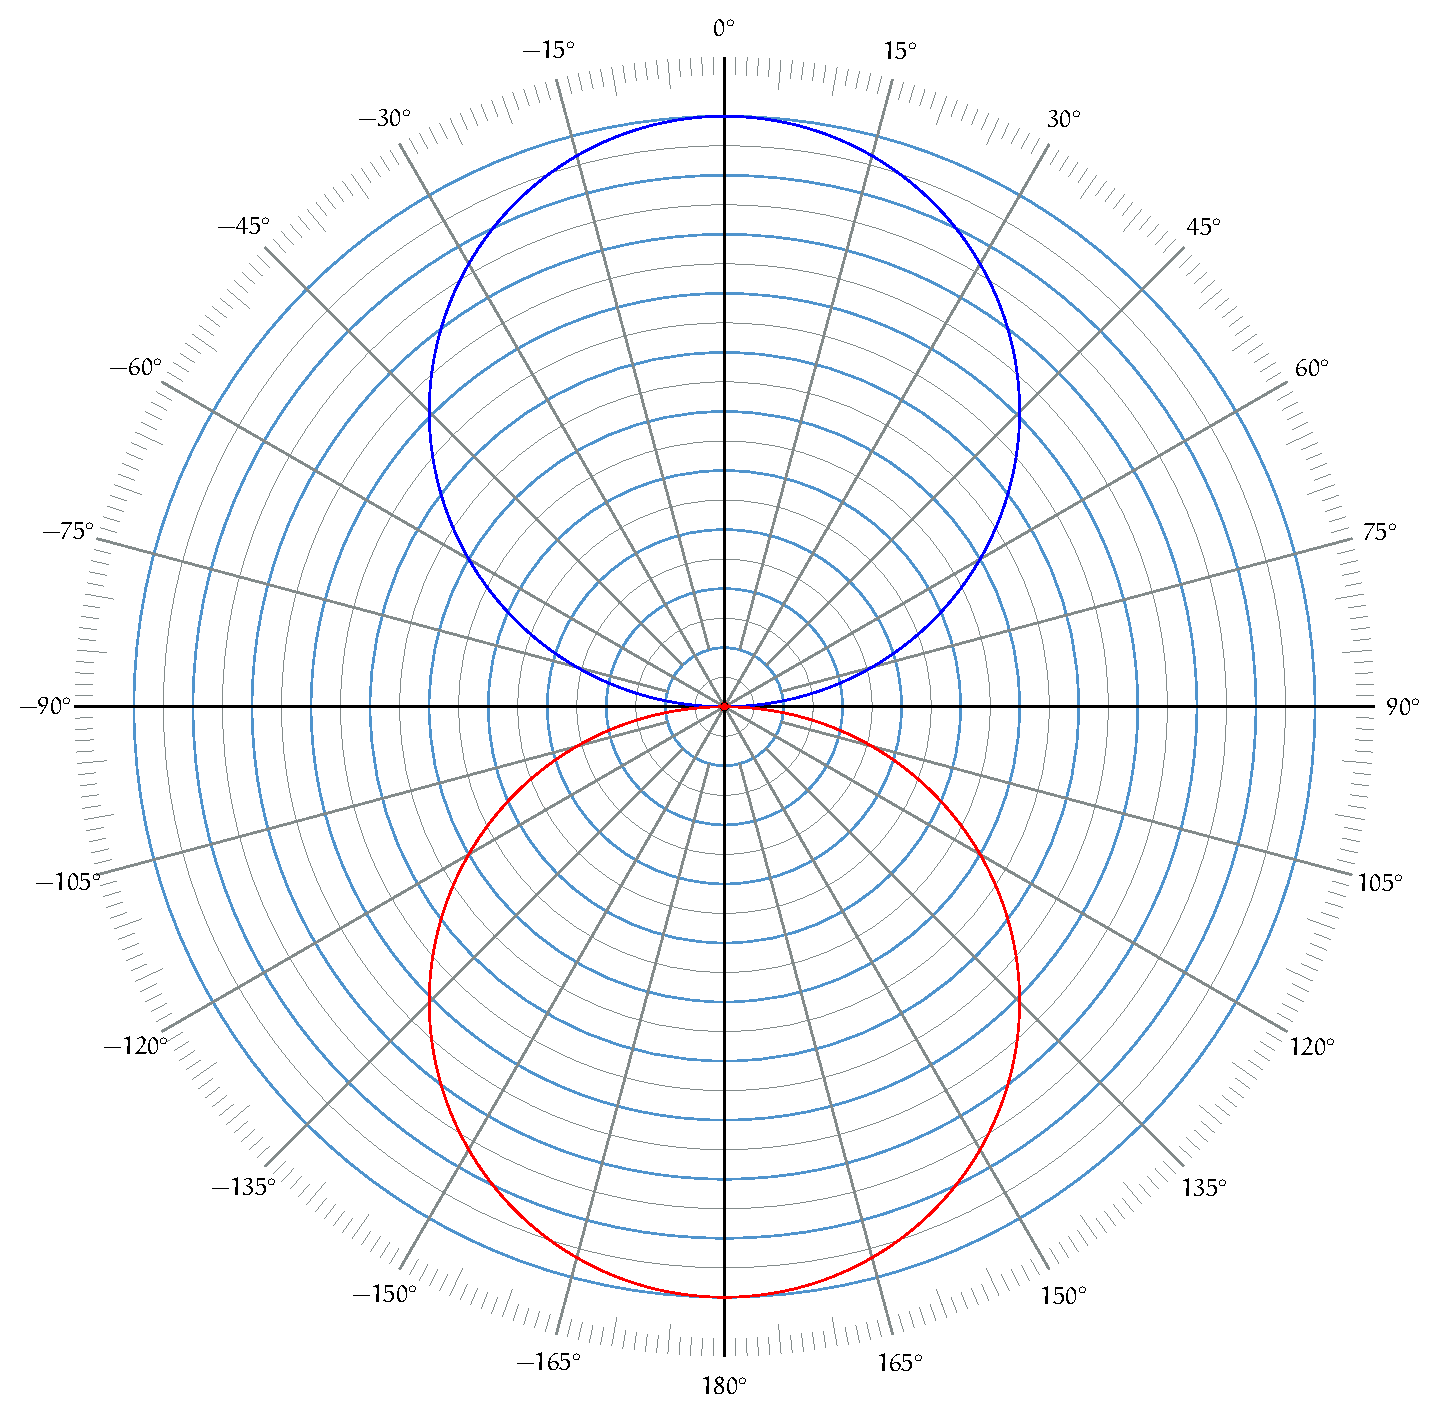
\includegraphics[width=\linewidth]{microphone-polar-patterns/fig8}\end{minipage}} \\
                & $0$          & $+$ & $1$                  & \\
                & $-\infty$    & $+$ & $0dB$            & \\ %20*log10(g)
& \\
\end{tabular}
\end{center}
\label{tab:polarcoef}
\end{table}

\clearpage

\begin{figure*}[h]
    \centering
    \begin{subfigure}[t]{0.48\textwidth}
        \centering
        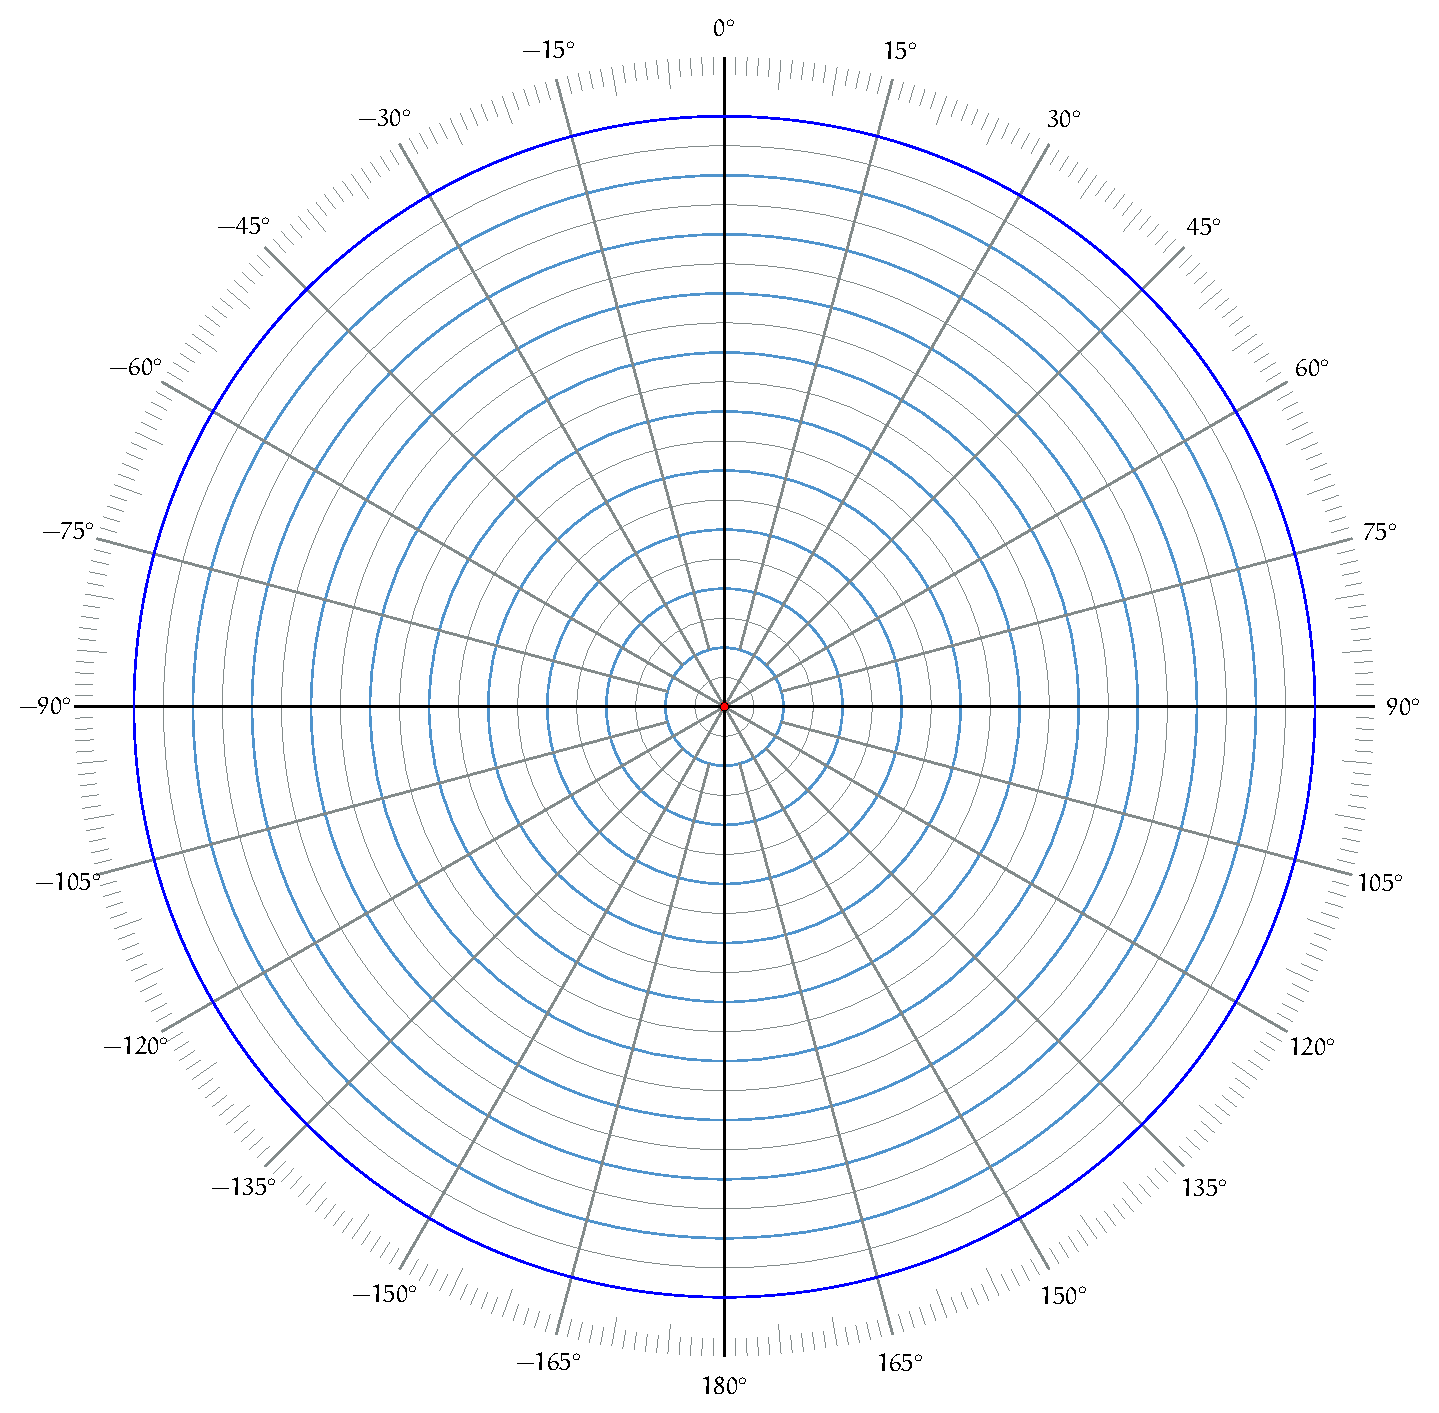
\includegraphics[height=6cm]{microphone-polar-patterns/omni}
        \caption[]{non-direzionale}% \\ Eq: $1(x)$}
        \label{pol:omni-p}
    \end{subfigure}%
    ~
    \begin{subfigure}[t]{0.48\textwidth}
        \centering
        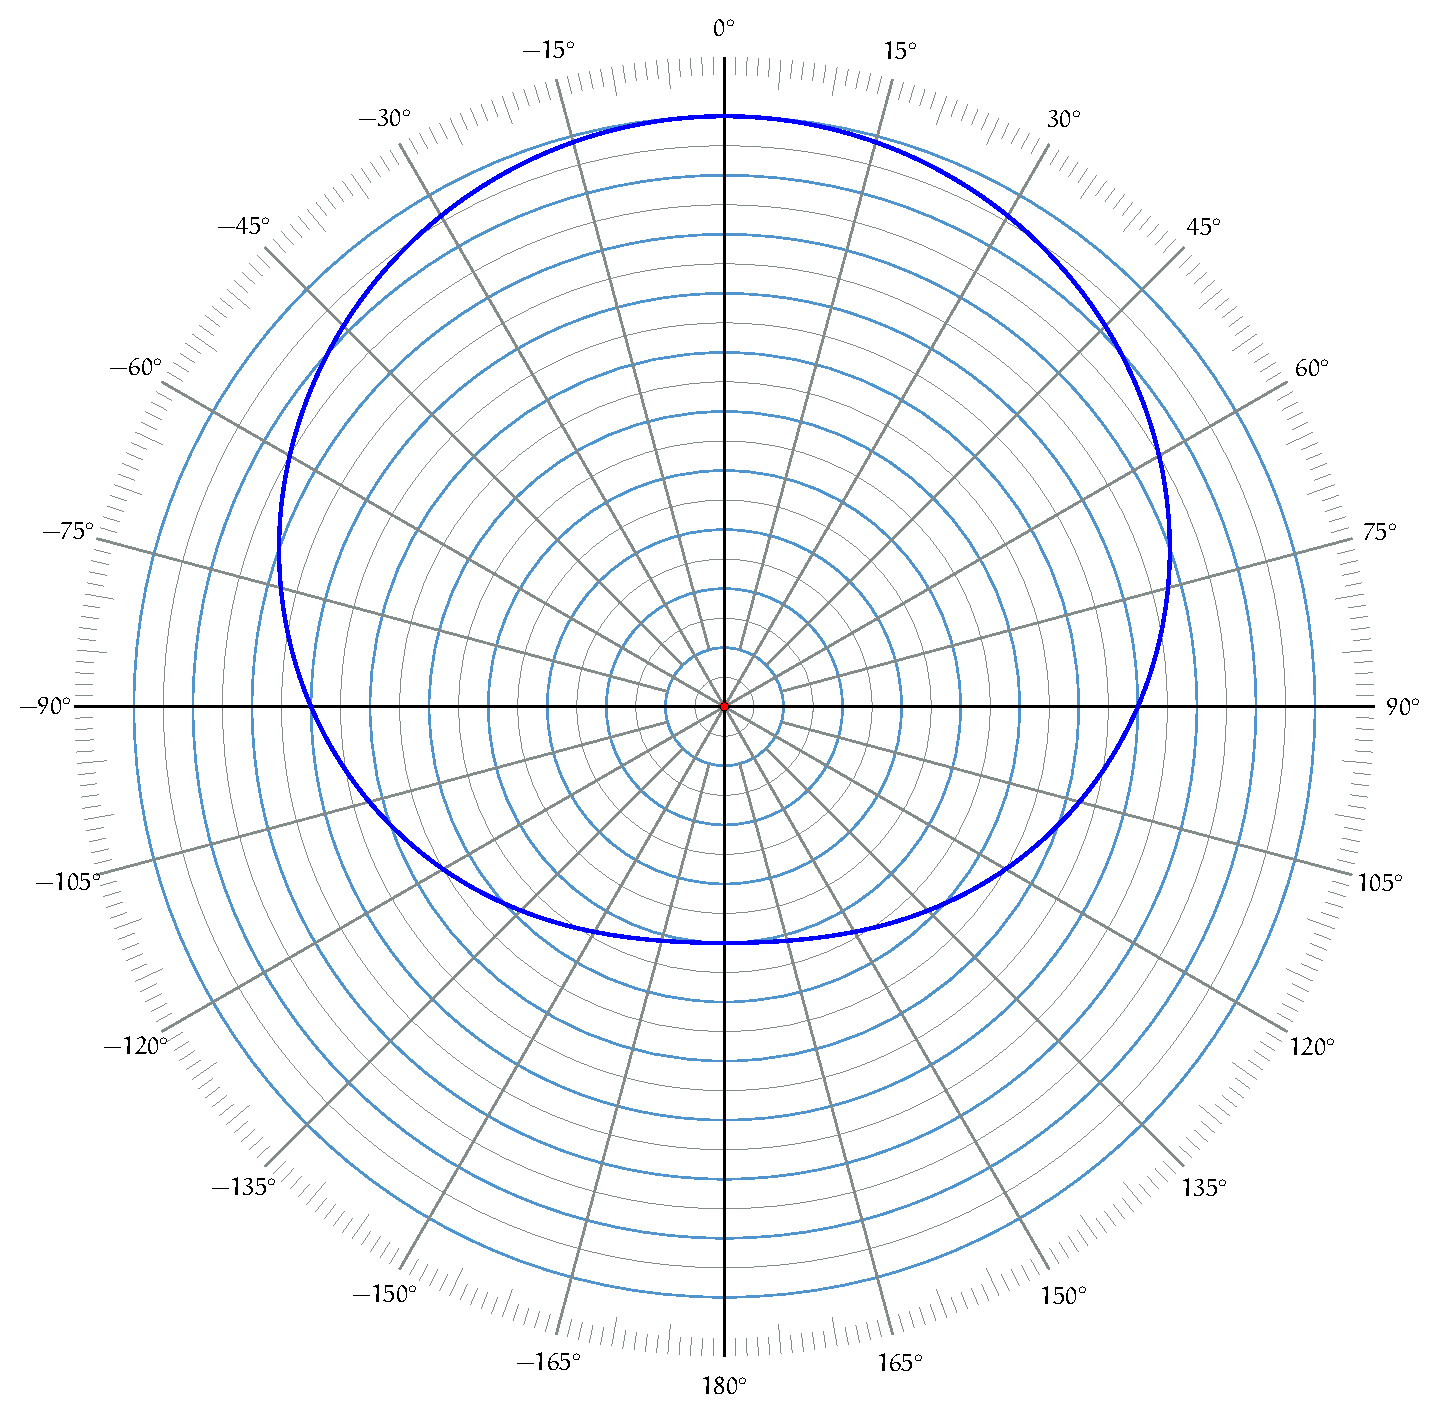
\includegraphics[height=6cm]{microphone-polar-patterns/subcardioid}
        \caption[]{subcardioide}% \\ Eq: $0.75(x)+0.25(x\cos\theta)$}
        \label{pol:sub-p}
    \end{subfigure}
    \\
    \begin{subfigure}[t]{0.48\textwidth}
        \centering
        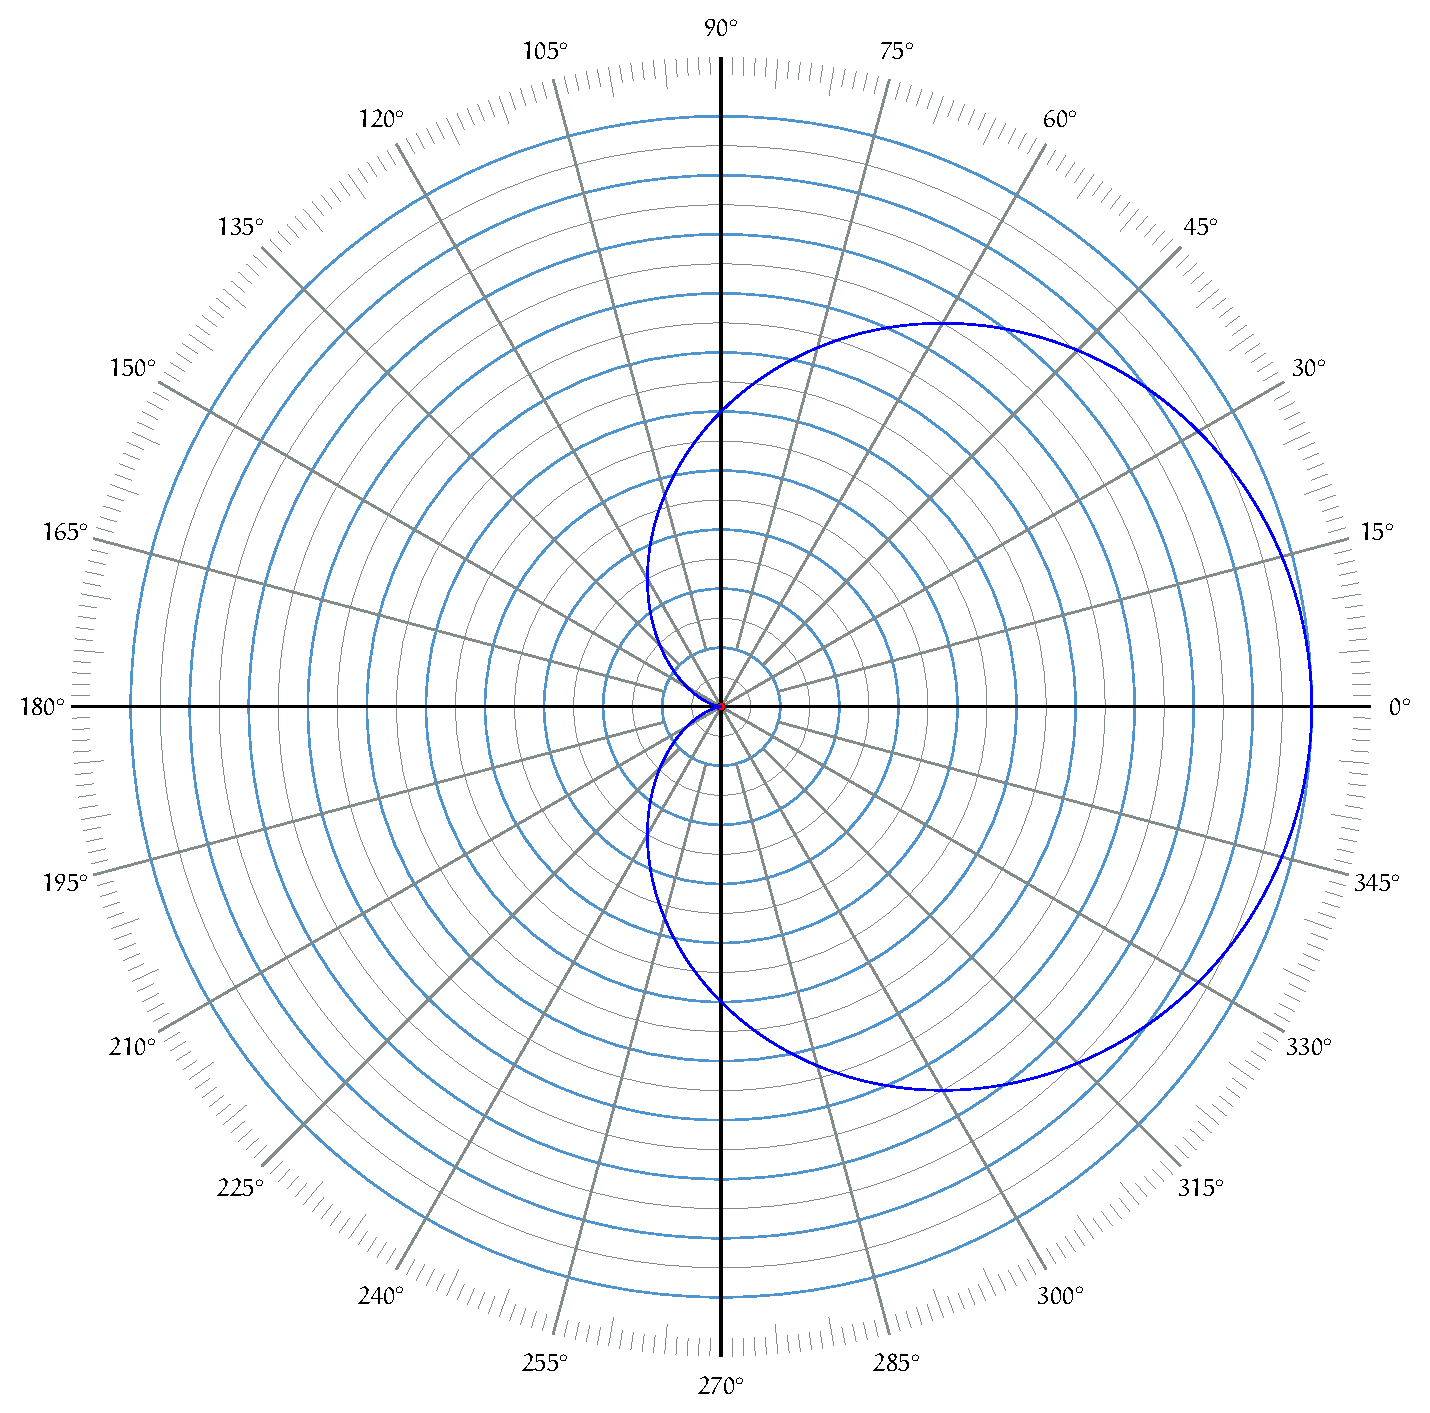
\includegraphics[height=6cm]{microphone-polar-patterns/cardioid}
        \caption[]{cardioide}% \\ Eq: $0.5(x)+0.5(x\cos\theta)$}
        \label{pol:cardio-p}
    \end{subfigure}
    ~
    \begin{subfigure}[t]{0.48\textwidth}
        \centering
        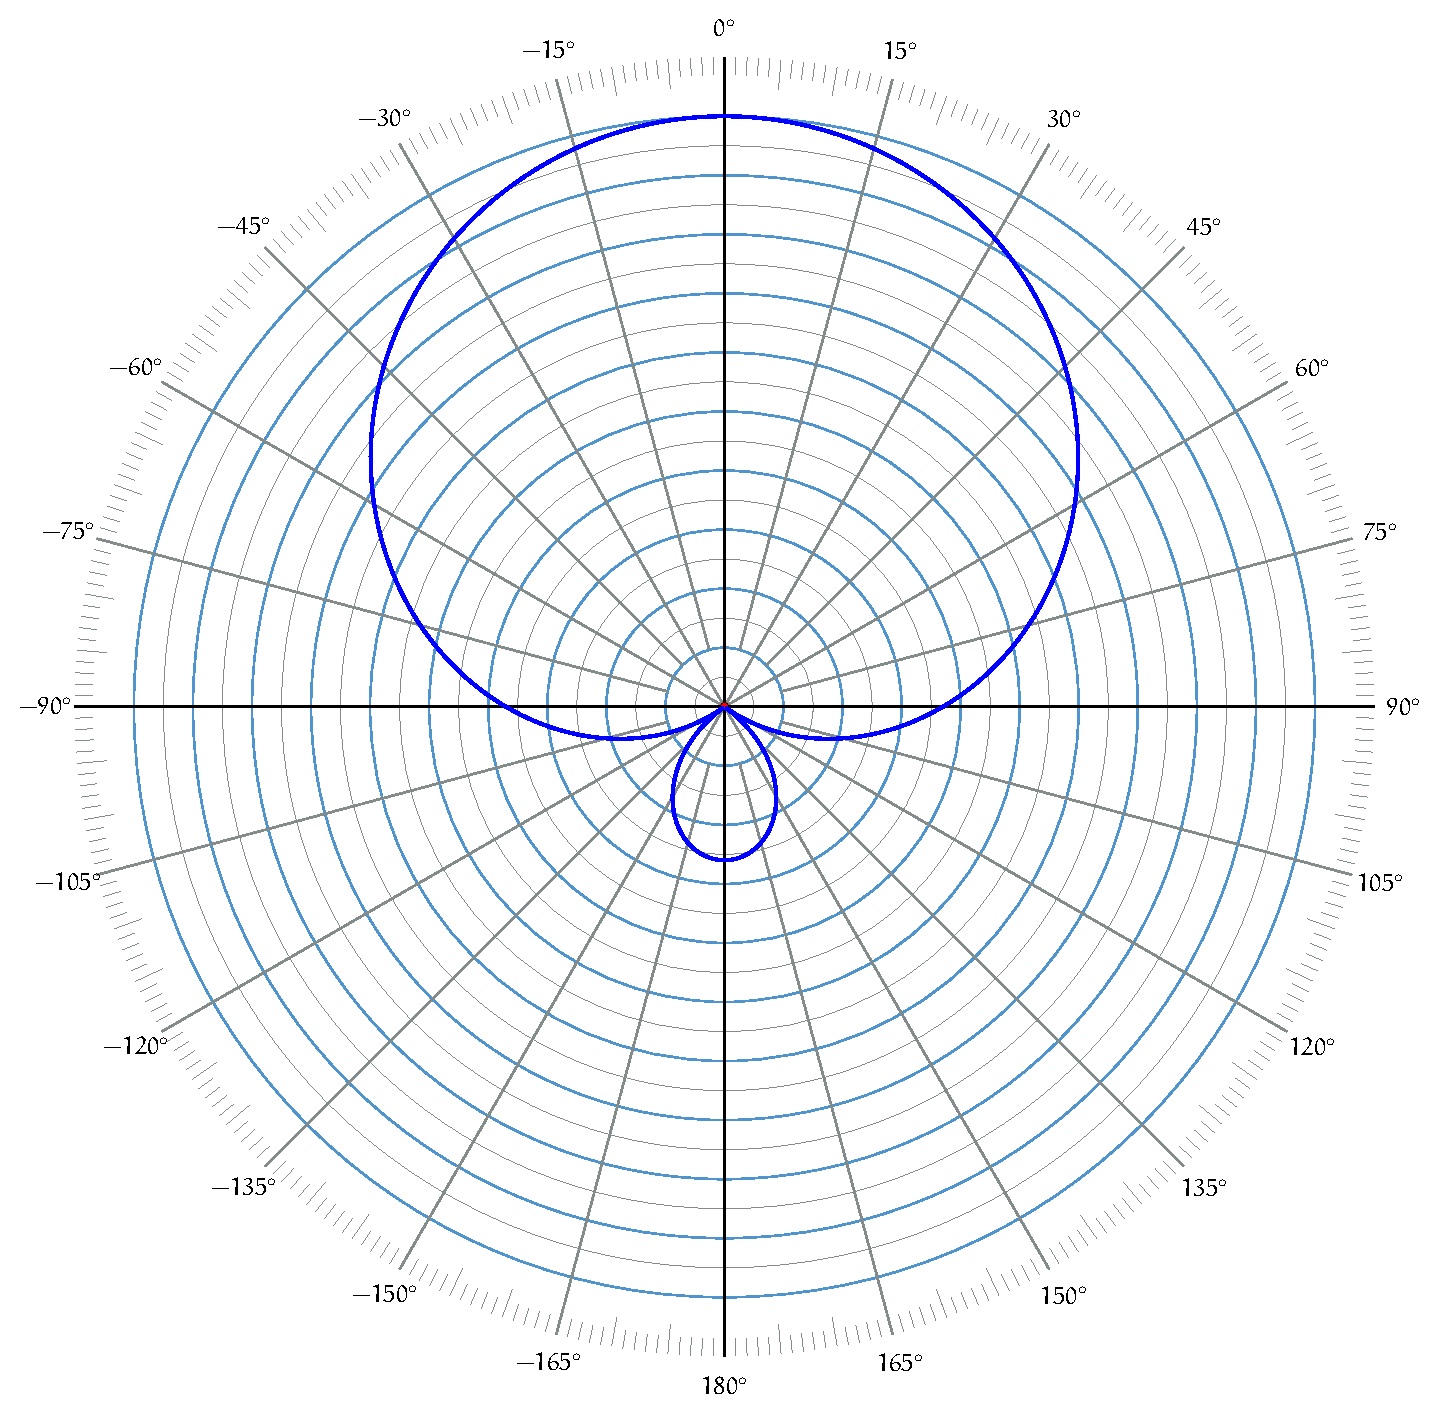
\includegraphics[height=6cm]{microphone-polar-patterns/supercardioid}
        \caption[]{supercardioide}% \\ Eq: $0.37(x)+0.63(x\cos\theta)$}
        \label{pol:super-p}
    \end{subfigure}
    \\
    \begin{subfigure}[t]{0.48\textwidth}
        \centering
        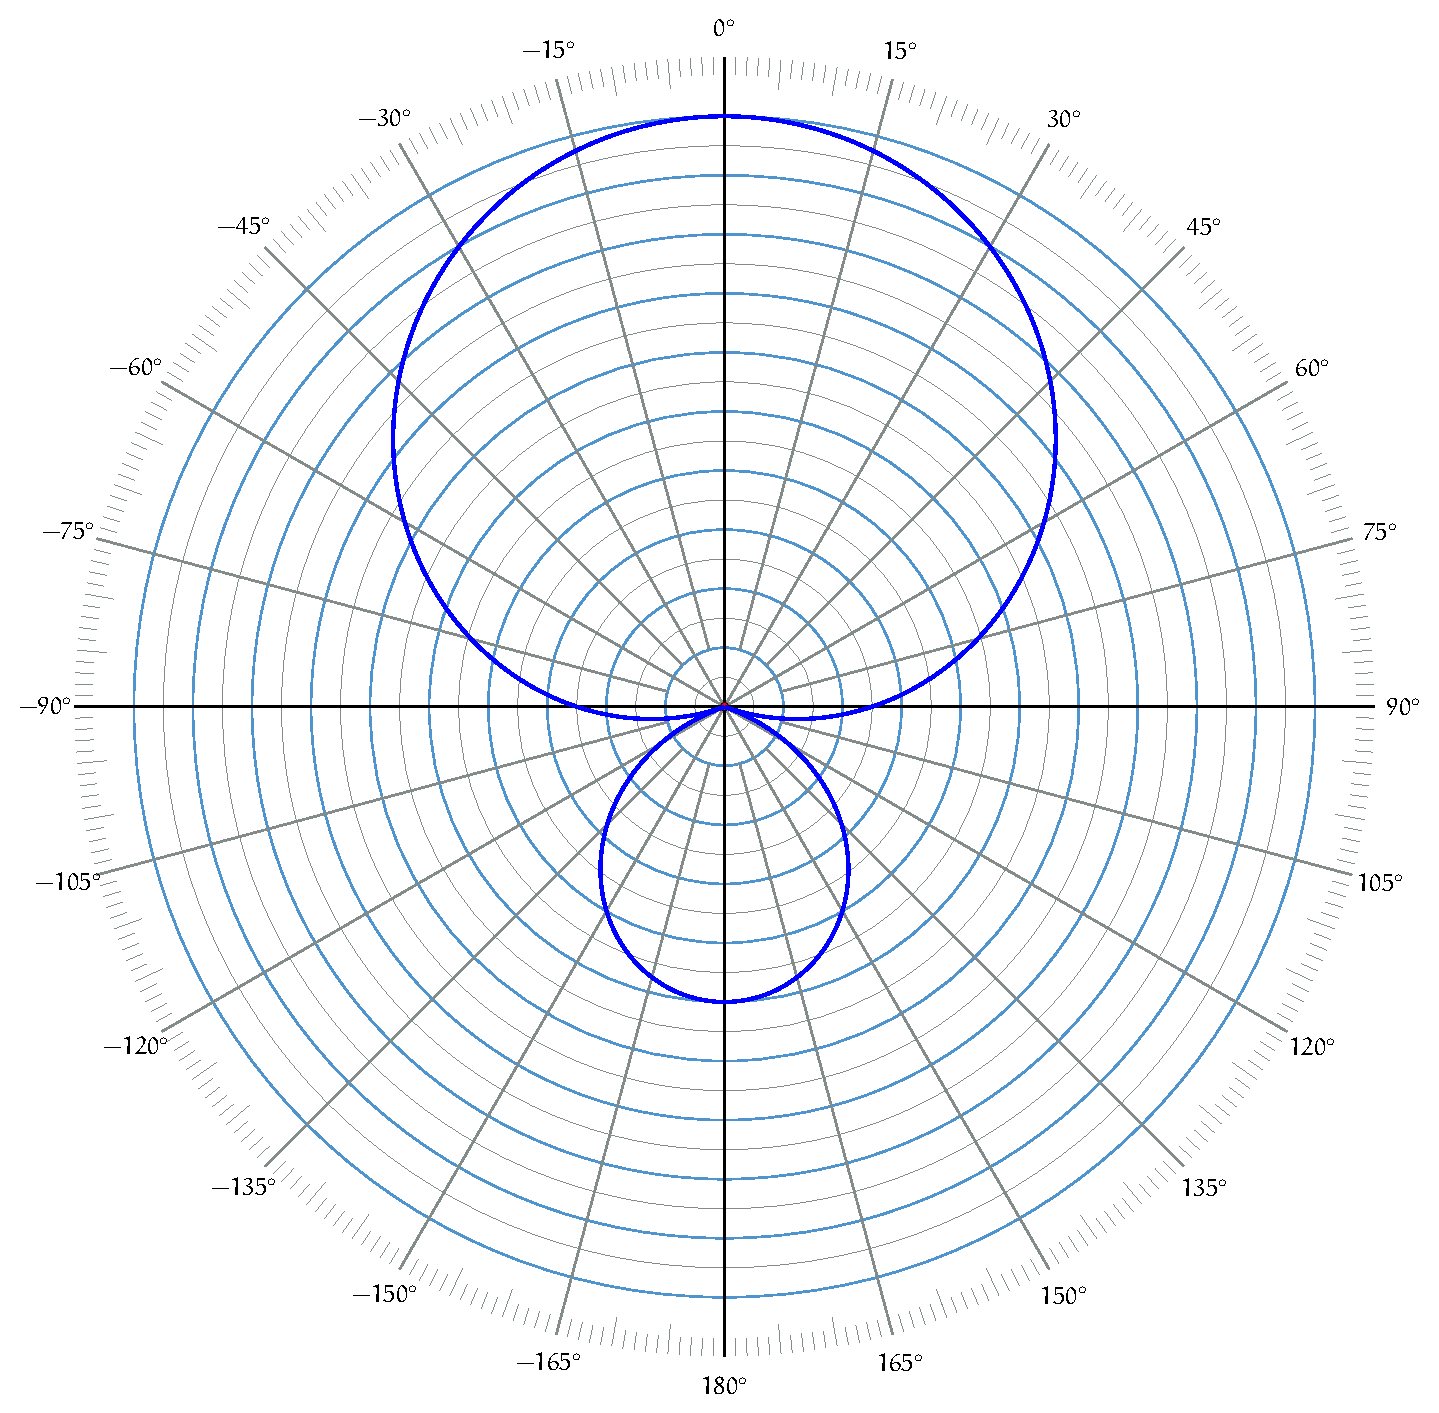
\includegraphics[height=6cm]{microphone-polar-patterns/hypercardioid}
        \caption[]{ipercardioide}% \\ Eq: $0.25(x)+0.75(x\cos\theta)$}
        \label{pol:iper-p}
    \end{subfigure}
    ~
    \begin{subfigure}[t]{0.48\textwidth}
        \centering
        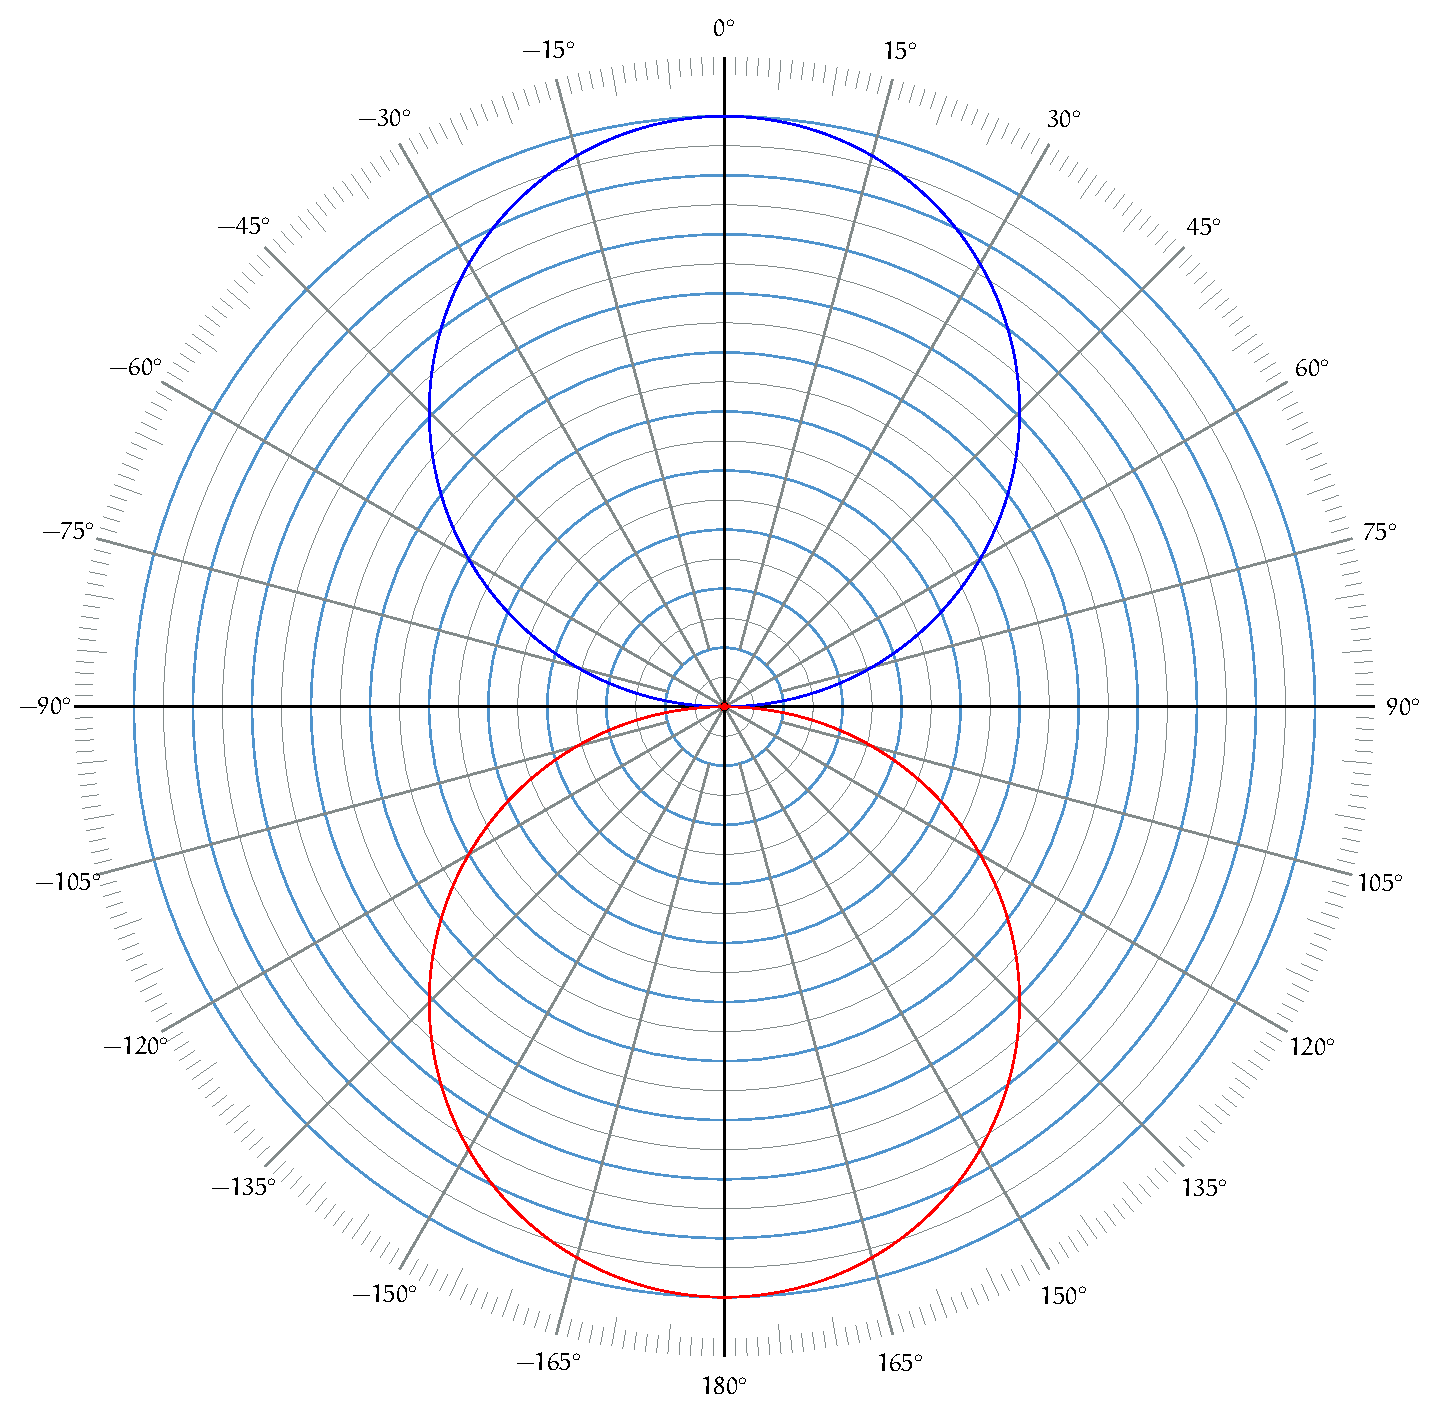
\includegraphics[height=6cm]{microphone-polar-patterns/fig8}
        \caption[]{figura-8}% \\ Eq: $1(x\cos\theta)$}
        \label{pol:fig8-p}
    \end{subfigure}
    \caption[]{Le principali figure polari ottenute mediante la calibrazione dei
    coefficienti di ampiezza della componente non-direzionale (fig. \ref{pol:omni-p}) e
    e bidirezionale (fig.\ref{pol:fig8-p}).}
    \label{pol:princicpali}
\end{figure*}
